\documentclass{ieeeaccess}
\usepackage{cite}
\usepackage{amsmath,amssymb,amsfonts}
\usepackage{algorithm}
\usepackage{algpseudocode}
\usepackage{graphicx}
\usepackage{textcomp}
\usepackage{mathtools}

\usepackage{subfigure}
\usepackage{caption,setspace}
\captionsetup{font={sf,small,stretch=0.80},labelfont={bf,color=accessblue}}

\usepackage{multirow} % added by user
\usepackage{array} % added by user
\usepackage{bigstrut} % added by user
\usepackage{setspace} % added by user
\def\BibTeX{{\rm B\kern-.05em{\sc i\kern-.025em b}\kern-.08em
    T\kern-.1667em\lower.7ex\hbox{E}\kern-.125emX}}
\begin{document}
\history{Date of publication xxxx 00, 0000, date of current version xxxx 00, 0000.}
\doi{10.1109/ACCESS.2017.DOI}

\title{Traffic Optimized Content Precaching Scheme based on Tolerable Delay Time in Content-Centric Vehicular Networks}
\author{\uppercase{Youngju~Nam}\authorrefmark{1}, %\IEEEmembership{Fellow, IEEE},
\uppercase{Hyunseok~Choi\authorrefmark{1}, Yongje~Shin\authorrefmark{1}, Seungmin Oh\authorrefmark{2} \IEEEmembership{Member, IEEE} and Euisin~Lee\authorrefmark{3}}.
%\IEEEmembership{Member, IEEE}
}

\address[1]{Research Institute for Computer and Information Communication, Chungbuk National University, Cheongju 28644, Republic of Korea (e-mail: imnyj@chungbuk.ac.kr; hschoi@chungbuk.ac.kr; yjshin@chungbuk.ac.kr)}
\address[2]{Department of Computer Science and Engineering, Kongju National University, Cheonan 31080, South Korea (e-mail: smoh@kongju.ac.kr)}
\address[3]{School of Information Communication Engineering, Chungbuk National University, Cheongju 28644 Republic of Korea}
\tfootnote{This research was supported by Chungbuk National University Korea National University Development Project (2022).}

\markboth
{Author \headeretal: Preparation of Papers for IEEE TRANSACTIONS and JOURNALS}
{Author \headeretal: Preparation of Papers for IEEE TRANSACTIONS and JOURNALS}

\corresp{Corresponding author: Euisin~Lee (e-mail: eslee@chungbuk.ac.kr).}

\begin{abstract}
The development of smart vehicles such as self-driving cars has resulted in an increased demand for content consumption in vehicles.
This demand for content, coupled with the improved quality of the content and the expanding resolution of the display, leads to a significant increase in mobile data traffics with larger sizes in content-centric vehicular networks (CCVNs). 
Since a single RSU cannot fully provide the larger size contents in its communication coverage due to its limited transmission rate, many studies on precaching contents have been actively conducted.
By considering only delay-sensitive contents, previous precaching schemes immediately precache contents in the next continuous RSUs on trajectories of vehicles through paying lots of traffics for reducing delays.
However, every application content in CCVNs might generally have a tolerable delay time to vehicles according to its characteristics related to service satisfaction. 
By considering the tolerable delay time, the already stored content on RSUs reached by vehicles within the tolerable delay time can be exploited to download the content without precaching. 
As a result, precaching of contents can be reduced and thus the traffics can be also reduced. 
To address this issue, we thus propose a Traffic Optimized Content Precaching (TOCP) scheme based on the tolerable delay time in CCVNs, which minimizes traffics consumed for delay-tolerant contents and decreases delays for delay-sensitive contents.
To do this, we first provide a numerical model to judge the precaching necessity by calculating the content provision possibility.
Next, we build a Delay-tolerant content Management Module (DMM) for managing the updated information and design new packet formats for reducing the movements of the large-size contents to achieve the optimization purpose of TOCP.
Then, we select Optimal Precaching RSUs (OPRs) by solving our optimization problem by using ILP.
Last, we provide a process for allowing only OPRs to participate in the content provision.
Through simulation results conducted in various environments, we demonstrate that TOCP minimizes the traffic and caching burden while maintaining high reliability in comparison with the previous schemes.

\end{abstract}

\begin{keywords}
Content-Centric Vehicular Networks, Content Precaching, Tolerable Delay Time, Optimization.
\end{keywords}

\titlepgskip=-15pt

\maketitle

\section{Introduction} \label{sec:introduction}
\PARstart{T}{he} development of smart vehicles such as self-driving cars, powered by advanced sensors and intelligent analysis tools, is a major milestone in the transportation industry \cite{Zhe2020}.
Smart vehicles enable them to drive safely on roads through their own trajectory with less human intervention \cite{yuan2018}.
In vehicles, drivers, as well as passengers, don't need to concentrate on driving much while they travel on their way so they have more free time to enjoy their life.
As a result, demands for various contents will be increased by vehicles and it makes mobile data traffics increase in vehicular networks \cite{Kumer2013, Pranav2019, Reichardt2002, Yen2020}.
Moreover, mobile data traffics are dramatically increased by the larger-sized contents due to their improved quality and the enlarged size of vehicles' display.
According to the Ericsson Mobility Report, total mobile network traffic, including fixed wireless access, is expected to nearly quadruple from around 115 EB per month by the end of 2022 to 453 EB per month by the end of 2028 \cite{Ericsson}.
Of this mobile data traffic, video traffic is estimated to account for about 70 percent of that, a share that is expected to increase to 80 percent by 2028.
Also, since a roadside unit (RSU) can not complete the provision of the content within its communication coverage due to the larger-sized content, a vehicle user suffers an access delay in bringing the content to the content server within the communication coverage of the next RSU.
Furthermore, due to the limited capacity of the base station (BS)'s wireless communication resources, the huge mobile data traffics cause delays like crowded places in vehicular networks because content packets are dropped due to overstack and are scheduled to postpone due to too many packets in the queue.
In the provision of delay-sensitive contents such as real-time streaming services and 3D games, packet delays directly affect the Quality of Service (QoS) for users through buffering and unstable connection.
Furthermore, in the case of driving assistance applications, it becomes a critical issue in terms of user safety due to the high speeds of vehicles.

As a strategy for solving the content delay and access problem, many studies \cite{Park2019, Ahani2018, AlNagar2019, Liang2018, Hou2019} on preaching have been actively conducted in Content-Centric Vehicular Networks (CCVNs) which are vehicular networks applied to  Content-Centric Networks (CCNs) \cite{Jacobson2009, zhang2014}.
In CCVNs, as an RSU can distributively solve content requests using caching storages of the RSU and other RSUs, it can solve the content delay problem by reducing BS's burden.
Also, the access delay problem can be solved by using precaching, which is to proactively cache requested contents on caching storage of nodes that requester vehicles will be encountered.
Since a requested content consists of a lot of chunks and thus the number of chunks that can be delivered within an RSU is limited due to the mobility of the requester vehicle, several studies in \cite{Zhe2020, Khelifi2018, Park2019} proposed schemes to calculate the number of chunks that have to be precached.
The schemes in \cite{Ahani2018, AlNagar2019, Liang2018} optimized the number of chunks that have to be precached while considering other limitations such as link capacity, storage, or buffer time.
Furthermore, by using deep reinforcement learning and $Q$--learning, the schemes in \cite{Hou2019, Zhu2019} tried to minimize the delay to provide the contents to requester vehicles.
However, most existing precaching schemes in CCVN focus on reducing the delays in the provision of delay-sensitive content (DSC) within the limited capacity of the BS's or RSU's wireless communication resources.
Imprudent precaching without considering RSUs that have already cached the requested content leads to increased traffic consumption on RSUs, which can exceed the capacity of backhaul links and wireless communication resources on RSUs.


To address this issue, research on reducing the traffic consumption has been studied \cite{Ostrovskaya2018, Marica2021, Amit2019}.
As an approach to do this, some schemes tried to reduce traffics consumed to access to content providers by precaching the popular content based on the content popularity prediction.
However, due to the limited storage capacity of RSUs, since all popular contents cannot be precached of RSUs, it is necessary for non-precached contents to access to the content providers.
As a result, this approach could not minimize the traffic consumption of backhaul links. 
As a different approach, some schemes considered Delay Tolerant Content (DTC) tolerable to delay (such as SW updates, backup services, 5 min for road congestion information, and 10 min for multimedia file sharing \cite{Lee2014, Chen2009}) and focused on increasing the reliability in the provision of small-sized contents in a sparse environment \cite{Qi2017, Vigneri2019, Xia2020}.
However, this approach is not effective in urban areas, where the demand for larger-sized contents is growing.
Moreover, by allowing infinite delays to reduce traffics, it decreases the reliability of content downloading because it violates the tolerable delay time due to the driving time of vehicles and the characteristics of contents.
As a result, the existing schemes for reducing the traffic consumption have not been entirely optimized in CCVNs.
Accordingly, a new scheme should be designed to minimize the traffic consumption while achieving a high level of reliability for delay-tolerant contents.

In this paper, we thus propose a scheme named Traffic Optimized Content Precaching (TOCP) based on the delay tolerable time in CCVNs.
The purpose of TOCP is to minimize the traffic consumed for delay-tolerant contents and to decrease the delay for delay-sensitive contents by using the saved traffic.
To accomplish this purpose, when a delay-tolerant content is requested by a vehicle, we first define a Precaching Available Area (PAA) by exploiting the tolerable delay time of the content and the mobility information of the vehicle.
Then, RSUs in the PAA are categorized into Already Cached RSUs (ACRs) with the content and Non-Cached RSUs (NCRs) without the content.
Next, we provide a numerical model to judge the precaching necessity of the delay-tolerant content by calculating the provision possibility for the delay-tolerant content.
The provision possibility calculation relies on the average transmission rate of each RSU in the PAA and the dwell time of the requester vehicle in the coverage of the RSU.
In TOCP, since the information such as the average transmission range of every RSU, the average speed of vehicles in the RSU, and the precaching road in the RSU needs to be real-time and efficiently updated for selecting Optimal Precaching RSUs (OPRs) for the content precaching, we next build a Delay-tolerant content Management Module (DMM) for managing the update information and conducting complex calculations for the optimization, and design new packet formats for reducing the movements of the large-size data packets for the content in order to achieve the information update process for the short delay and small traffic costs.
Then, we formulate an optimization problem for selecting OPRs based on the latest updated information and solve it by using the Integer Linear Programming (ILP) to minimize the traffic consumption, the traffic congestion on backhaul links, and the caching burden for holding the requested contents until the requester vehicle enters.
Lastly, we provide a process for allowing only OPRs to participate in the provision of the delay-tolerant content and to send only the first and the last chunks allocated to themselves to the requester vehicle for the content provision.
For evaluating the performance of TOCP, we implement the simulation using NS3 with the enhanced Manhattan mobility model such that vehicles accelerate with a Gaussian distribution and directionally shift on roads according to their trajectories to reflect a city scenario.
Through the simulation results conducted in various environments, we verify that the performance of the proposed scheme TOCP reaches to minimize the traffic consumption with achieving high reliability in comparison with two existing schemes, the closest scheme and the random scheme on selecting RSUs for precaching.


The remainder of the paper is organized as follows.
Section \ref{sec2} reviews the related work of precaching schemes and delay-tolerant content (DTC) in CCVNs.
In Section \ref{sec.net}, we describe the network model and overview of the proposed scheme called Traffic Optimized Content Precaching (TOCP).
Then, Section \ref{sec.prop} details the proposed scheme that minimizes traffic consumption for the DTC.
To validate the performance of the proposed scheme, Section \ref{sec.s} conducts simulations reflecting various environments and explains simulation results.
Finally, Section \ref{sec.c} concludes the paper.

\section{Related Work} \label{sec2}
% CCVN
The traditional IP-based network has some limitations that disturb the efficient delivery of large-sized content, especially in vehicular networks.
These limitations include limited bandwidth, high latency, and frequent packet loss, which reduce the reliability and QoS of the network.
In vehicular networks, the main challenge issue is to reduce delays in providing various services to vehicles because the delays are directly connected to vehicle users' safety and QoE.
To solve the issue, many researchers have studied content-centric vehicular networks (CCVN), which applied the concept of content-centric networks (CCN \cite{Jacobson2009, zhang2014}) to vehicular networks \cite{Amadeo2012, Su2017, Wang2019}.
By focusing on the content itself instead of the location of the content based on IP, CCVN can reduce traffic overhead and delays due to existing IP-based networks.
In CCN, all node has storage device to cache the content in the progress of forwarding or providing the content according to their protocol.
Thus, in CCVN which is applied that concept, all roadside units (RSUs) is equipped with their storage device and all vehicles include storage devices in their onboard units (OBU).
Several studies have been studied about how CCN can be utilized in vehicular networks to improve performance \cite{Amadeo2012, Su2017, Wang2019}.
Amadeo~et~al.~\cite{Amadeo2012} had a view that a CCN-like approach outperforms the legacy TCP/IP protocol suite and well copes with dynamic, short-lived, and intermittent connectivity in vehicular environments. Thus, they evaluated the performance of a broad simulation study aiming at evaluating the effectiveness and efficiency of the proposed content-centric vehicular networking architecture under a variety of different traffic loads, vehicle densities, and content popularity settings.
Su~et~al.~\cite{Su2017} presented a novel framework for a content-centric vehicular network (CCVN). In that framework, they presented an integrated algorithm to deliver content to vehicles with the help of content-centric units, which is that content can be stored according to their priorities determined by vehicle density and content popularity. In their CCVN, by introducing a content-centric unit, contents exchanged between vehicles can be managed based on their naming information. Also, pending interests are updated based on the analysis of the transmission ratio and network topology.
Wang~et~al.~\cite{Wang2019} proposed an IP-based vehicular content-centric networking framework, which focuses on acquiring content related to a given position. In this framework, a requester acquires contents in the address-centric unicast way, so the contents can be returned to the requester without depending on reverse paths. Moreover, content in a given position is obtained from the nearest provider, so the content acquisition cost can be reduced.
% CCVN의 한계점
However, even if the provided and forwarded content is cached, all content can not be cached due to the storage capacity limitation of the RSU.
Therefore, the requested content by the vehicle that newly enters has to be brought from the provider if the content has been not cached in this RSU's storage.
The access to the provider is increased because of the frequent handover due to the vehicle's high speed, and it causes access delay and degraded QoS.

% Precaching (Pop, Mob)
To reduce the access delay and improve the QoS in CCVN, the precaching scheme has been studied by many researchers \cite{Ostrovskaya2018, Marica2021, Amit2019, Zhe2020, Park2019, Khelifi2018}.
The precaching scheme is a technique that involves proactively caching the content that will be requested by the newly entering vehicles before the vehicle enters.
In the context of CCVN, the precaching scheme can be used to reduce the access delay to the provider when the vehicle enters, and to improve the reliability of content delivery to the requester vehicle.
There have been several approaches to precache the content: 1) prediction of the request based on the popularity of the content; 2) prediction of the requester vehicle's location based on its mobility.
First, precaching schemes based on request prediction have been studied, which are to precache the content that has a high probability of requesting before the vehicle requests \cite{Ostrovskaya2018, Marica2021, Amit2019}.
Ostrovskaya~et~al.~\cite{Ostrovskaya2018} proposed a new multi-metric content replacement policy (M2CRP) for content stores in NDN-driven VANETs. M2CRP considers three metrics to collectively encompass the requirements for the improved performance of VANET applications: the freshness of the content, the popularity, and the distance between the locations where the content was received and saved in content stores and the current location of the caching node.
Marica~et~al.~\cite{Marica2021} proposed a novel caching strategy, referred to as Diversity improved cAchiNg of popular Transient contEnts (DANTE) where vehicles autonomously decide which content is to be locally cached according to the content residual lifetime, its popularity, and the perceived availability of the same content in the neighborhood. They also design a set of minor modifications in the Named Data Networking (NDN) node architecture and packet fields to support DANTE operations. Caching decisions are taken by vehicles autonomously. Vehicles can find the majority of distinct fresh and popular content nearby, without flooding the network with content requests that have to reach the original source.
Dua~et~al.~\cite{Amit2019} proposed a content caching scheme based on a bloom filter model (that is the probability data structure) to improve efficient content distribution in CCVNs. The bloom filter model is used to achieve better time complexity and quicker content insertion, deletion, and search processes. Through the bloom filter model, the scheme allows vehicles to have the functionality of cache to support cooperative content distribution between them.

Subsequently, precaching schemes based on mobility prediction have been studied, which are to precache the content that will be requested by predicting the movement of vehicles \cite{Zhe2020, Park2019, Khelifi2018}.
Zhe~et~al.~\cite{Zhe2020} proposed a novel hierarchical proactive caching approach that considers both the future demands of autonomous vehicle users and their mobility. This approach uses the non-negative matrix factorization (NMF) technique to predict users’ preferences which are then used to predict users’ future demands by considering the historical popularity of videos. They calculate the number of video chunks for precaching by using the arrival and departure time of the user at an edge node based on its current velocity vector. They consider not only the predicted ratings, but also the previous popularity of videos to predict the users’ future demands.
Park~et~al.~\cite{Park2019} proposed a mobility-aware distributed proactive caching scheme in CCVNs. To reduce the redundancy and the burden of precaching for multiple candidate next RSUs from the current RSU, the proposed scheme distributes the whole of the intended content to each of them as much as the mobility probability of the requester vehicle about each candidate next RSU, which means the probability to move to the candidate next RSU from the current RSU by the requester vehicle based on the Markov Model. They calculate the maximum number of chunks using the constant vehicle speed, and these chunks are distributively precached to each of the candidate next RSUs to which the requester vehicle may travel.
Khelifi~et~al.~\cite{Khelifi2018} proposed an optimized precaching scheme called PCMP for VANETs on the top of the NDN architecture, which predicts the next arrival RSU based on the LSTM module and precaches the intended content on the RSU. They calculated the number of chunks using the current velocity of the requester vehicle and the distance of the path at the coverage of RSU. Then, PCMP divides the intended content into chunks, then calculates the number of chunks required to be precached and downloaded in the next RSU. For the calculation, it exploits the connectivity duration of the requester vehicle within the coverage of the RSU and the link bandwidth between the vehicle and the RSU.
The existing precaching schemes have limitations.
In the precaching scheme based on request prediction, an RSU can not precache all popular content, so it couldn't minimize access to the provider because the requested content has to be brought from the provider if the RSU doesn't have the content.
Also, in the precaching scheme based on mobility prediction, because the delay-tolerant content (DTC) was not considered, the RSU increases too much burden on the backhaul links by pre-caching the requested DTC at the RSU which is consuming much traffic to provide other content to other vehicles even if the requested DTC does not need to be rushed to be provided.
Consequently, the existing precaching scheme could not optimize the performance in terms of access delay and traffic overhead.

Therefore, by minimizing the traffic consumption for delay-tolerant content, we can get sufficient link capacity for delay-sensitive content.
In the case of the delay-tolerant content (such as SW updates, backup services, 5 min for road congestion information, and 10 min for multimedia file sharing \cite{Lee2014, Chen2009}), because it does not need to rush to be downloaded, it can be downloaded using the RSUs that already cached it without additional traffic.
But, the CCVN approaches for the delay-tolerant content have been studied in a very early stage \cite{Qi2017, Vigneri2019, Xia2020, Prates2019, Aung2023}.
\cite{Qi2017} made the routing graph for reducing backhaul link overhead and improving reliability by using mobility prediction based on vehicle’s mobility patterns in Delay-Tolerant Network(DTN)-enabled vehicular ad hoc networks.
It selected the least-cost route with limited reliability by using a spatio-temporal graph.
\cite{Vigneri2019} minimized the cellular cost by using buffers of the requested content that is already cached when the requester pedestrians stayed within the coverage area of an RSU.
It considered the situations of delay-tolerant content and not delay-tolerant content to provide the content to requester pedestrians by using the neighboring vehicles as helpers.
These approaches considered the small data packet in a sparse environment.
Thus, they are not suitable for the vehicular network which has an increased demand for larger-sized content.
\cite{Xia2020} minimized the energy consumption and delays for users by using hierarchical networks that consisted of fog in the under layer, cloud in the upper layer, and an SDN server that can control those layers.
Because the relationship between energy consumption and delays is a trade-off, their delay-tolerant transmission scheme focused on minimizing energy consumption.
In providing the delay-tolerant content, the existing schemes did not consider the tolerable delay time, which comes from the content characteristics and the requester vehicle's driving time.
Then, the reliability of the content download is reduced because the requester vehicle can not complete downloading the delay-tolerant content within the allowed time.

In this paper, we proposed the precaching scheme to maximize the link capacity for DSC by minimizing the traffic consumption for DTC based on mobility prediction and communication information update.
To reach the purpose, our contribution is as follows:
\begin{itemize}
\item To prevent reckless precaching, we classify the DTC and the DSC according to the delay tolerance characteristic.
Through the classified DTC, we can cut the not necessary provision and precaching of delay-tolerant content and it denotes the traffic consumption save.
\item For the guarantee of content download completion, we consider the tolerable delay time in the provision of the DTC.
The tolerable delay time in CCVN is defined as the maximum time that a content should take to be fully downloaded and available for the requester vehicle, considering its characteristics and the driving time of the vehicle.
By completing the download of the DTC within the tolerable delay time, the reliability is improved.
\item We designed the DTC management module (DMM) for prediction improvement and complex calculations.
DMM has a better prediction accuracy because of updating the communication information of RSUs via packets.
By improved prediction accuracy, the traffic consumption for the provision of DTC is minimized while high reliability.
\item Additionally, DMM solves the optimization problem based on the updated information by using Integer Linear Programming (ILP).
DMM which is equipped in each content server has enough computing resources.
Through the sufficient computing resource of the server, DMM can select the optimal precaching RSUs that will be attended for the provision of DTC to minimize traffic consumption, traffic congestion, and caching burden.
\end{itemize}

\section{Network Model and Scheme Overview} \label{sec.net}
In this section, we provide the network model and the overview of the proposed scheme named TOCP. 
We first present the network model of TOCP and then describe the overview of TOCP in the following subsections, respectively.

\subsection{Network Model}
In this subsection, we describe the network model of TOCP.
In this paper, TOCP considers a content-centric vehicular network for providing content services to vehicle users as its network model as shown in Fig. \ref{fig:ov}.
To support this network model, We have several assumptions about the network architecture and the behavior of vehicles and content servers.
Specifically, we first assume that every intersection is equipped with an RSU that provides Delay-Tolerant Contents (DTC) and Delay-Sensitive Contents (DSC) from content servers to vehicles over IEEE WAVE communications \cite{WAVE}, and all the RSUs and content servers are connected via fiber links.
Additionally, we assume that content servers of the requested content by vehicle users are equipped with a DTC Management Module (DMM) to update RSU's communication capacity information and solve the optimization problem using the updated information.
Since the locations of all RSUs are fixed and difficult to change, we assume that the DMM knows the locations of all RSUs and has a map with their locations on the roads.

The generation of a new request from each vehicle is determined every unit of time according to a Poisson distribution.
The request for content follows Zipf's law \cite{Zipf}, where popular content is more likely to be requested.
The popularity of content is determined differently by DTCs and DSCs.
The vehicles can request or receive DTC as a background service while being served DSC.
A requested DTC by a requester vehicle has a unique tolerable delay time, which varies based on the characteristic of the requested content and the driving time of the requester vehicle.
Each vehicle has its destination and travels along the shortest route to the destination by passing several RSUs at an average speed based on a Gaussian distribution depending on road conditions.
When the provided or forwarded content is cached at the content store (CS) of each intermediate RSU, old content is more likely to be replaced because of the storage capacity limitation of an RSU.
Every RSU belongs to $\{R_{1}, \cdots, R_{J}\}$ and $j$-th RSU is $R_{j}\in\{R_{1}, \cdots, R_{J}\}$.
Every vehicle belongs to $\{V_{1}, \cdots, V_{I}\}$ and $i$-th vehicle is $V_{i}\in\{V_{1}, \cdots, V_{I}\}$.
Every content belongs to $\{C_{1}, \cdots, C_{C}\}$ and $c$-th content is $C_{c}\in\{C_{1}, \cdots, C_{C}\}$.
For computational simplicity, we also assume that all content is divided into the same-sized chunks, where chunks belong to an ordered set $\{1, \cdots, n_{c}, \cdots, N_{c}\}$.
Then, we denote that the size of one chunk is $s$.

\begin{figure}[ht]
    \centering
    
\includegraphics[width=\columnwidth]{./figure/overview.png}
    \caption{The network model and the overview of TOCP.}
    \label{fig:ov}
\end{figure}


\subsection{Scheme Overview}
In this subsection, we describe the overview of TOCP based on the network model shown in Fig. \ref{fig:ov}.
When a new request for a DTC or a DSC $C_{c}$ is made by a vehicle $V_{i}$, it sends an $Interest$ packet containing its mobility information for downloading the content $C_{c}$ to the RSU $R_{j}$ in which it located.
The mobility information of $V_{i}$ includes its current location, velocity, and trajectory.
On receiving the $Interest$ packet of $V_{i}$, $R_{j}$ checks with the mobility information of $V_{i}$ whether $V_{i}$ can complete the provision of the requested content $C_{c}$ within the communication range of $R_{j}$ based on its average transmission rate.
The average transmission rate of $R_{j}$ is calculated as follows based on historical data for an hour.
\begin{equation}
    r_{j}(t) = \cfrac{\sum_{q=0}^{t_{max}}r_{j}(t-q)}{t_{max}},
    \label{eq1}
\end{equation}
where $r_{j}(t)$ is the average transmission rate of $R_{j}$ at the time $t$ and $t_{max}$ is the maximum historical time of 3600 seconds.
$R_{j}$ updates the average speed $v_{j}(t)$ of vehicles within the coverage of this RSU using the same principle as updating the $r_{j}(t)$.
If the provision of $C_{c}$ can be completed, $R_{j}$ immediately provides it according to the basic CCVN procedure to prevent additional complicated procedures.
Based on the basic CCVN procedure, if $C_{c}$ is already cached in the CS of $R_{j}$, it is immediately provided through $Data$ packets from $R_{j}$ to $V_{i}$ within the communication range of $R_{j}$.
Otherwise, the $Interest$ packet is stored in the Pending Interest Table (PIT) and further is forwarded based on the Forwarding Information Base (FIB) to download $C_{c}$ to the content server or an RSU which has $C_{c}$.

If the RSU $R_{j}$ can not complete the provision of the requested content $C_{c}$ to the requester vehicle $V_{i}$, it verifies that $C_{c}$ is DTC or DSC.
If $C_{c}$ is DSC, $R_{j}$ sends a $Precaching$ packet to the next RSU $R_{(j+1)}$ based on the vehicle's mobility information so that $R_{(j+1)}$ can precache $C_{c}$ to minimize delay by providing the content immediately when $V_{i}$ enters the communication range of $R_{j+1}$. 
On the other hand, if $C_{c}$ is DTC, $R_{j}$ sends a $Request$ packet to the content server of $C_{c}$ to minimize traffic consumption.
When the content server receives the $Request$ packet, it moves the packet to its DMM.
Based on the mobility information of $V_{i}$ and the tolerable delay time $t^{i,c}_{tol}$ of $C_{c}$ by $V_{i}$, the DMM defines the Precaching Available Area $PAA^{i,c}$ that $V_{i}$ will travel within $t^{i,c}_{tol}$.
Then, using the location information of RSUs, the DMM finds out the Precaching Available RSUs $\{PAR^{i,c}_{1}, \cdots, PAR^{i,c}_{k}, \cdots, PAR^{i,c}_{K}\}$ which are belonged in $PAA^{i,c}$ and thus are encountered by $V_{i}$ during $tol^{i,c}_{tol}$.
The DMM makes the instant table for providing $C_{c}$ to $V_{i}$ and adds an ID of each $PAR^{i,c}_{k}$ to the table.
To find out how much load each $PAR^{i,c}_{k}$ spends to prepare $C_{c}$, the DMM sends an $Information$ $Request$ packet to the ID of each $PAR^{i,c}_{k}$.
If $PAR^{i,c}_{k}$ already caches $C_{c}$, it is classified as an Already Cached RSU $ACR^{i,c}_{k}$ and replies through sending an $Information$ $Reply$ packet to the DMM.
The $Information$ $Reply$ packet includes the average speed $v_{ACR^{i,c}_{k}}(t)$ of vehicles within the coverage of $ACR^{i,c}_{k}$, the average transmission rate $r_{ACR^{i,c}_{k}}$ and the load value $load_{ACR^{i,c}_{k}}(c)$ of $ACR^{i,c}_{k}$.
The average speed $v_{ACR^{i,c}_{k}}(t)$ of vehicles within the coverage of $ACR^{i,c}_{k}$ is defined as follows:
\begin{equation}
    v_{ACR^{i,c}_{k}}(t) = \cfrac{\sum_{q=0}^{t_{max}}v_{ACR^{i,c}_{k}}(t-q)}{t_{max}}.   \label{eq2}
\end{equation}

$ACR^{i,c}_{k}$ receives the speed of a vehicle within its coverage by beacon message, then it statistically averages them at each time $t$.
Since $load_{ACR^{i,c}_{k}}(c)$ is the burden value to bring $C_{c}$ at $ACR^{i,c}_{k}$, it is 0 in this case.
However, if $PAR^{i,c}_{k}$ does not cache $C_{c}$, it is classified as a Non-Cached RSU $NCR^{i,c}_{k}$.
Then, $NCR^{i,c}_{k}$ makes a new $Instant$ $Interest$ packet to know its load value $load_{NCR^{i,c}_{k}}(c)$.
According to the CCVN procedure, it forwards the $Instant$ $Interest$ packet to an RSU that has $C_{c}$ based on its FIB.
When the RSU $R_{m}$ that has cached $C_{c}$ receives the $Instant$ $Interest$ packet from its previous RSU $R_{(m-1)}$, it checks the traffic link usage ratio $U_{m(m-1)}(t)$, which is the usage ratio of the link from $R_{m}$ to $R_{(m-1)}$ at the time $t$.
Therefore, $U_{m(m-1)}(t)$ can be a value between 0 and 1 as the ratio of the link's traffic consumption to the link's maximum capacity.
The RSU adds the link usage burden value $D_{m(m-1)}(t)$ to $load_{NCR^{i,c}_{k}}(c)$ and puts $load_{NCR^{i,c}_{k}}(c)$ in the $Instant$ $Data$ packet, where $D_{m(m-1)}(t)$ is the burden to use the link between $R_{m}$ and $R_{(m-1)}$.
Since $D_{m(m-1)}(t) = (1-U_{m(m-1)}(t))^{-1}$, the link that is being used 100 \% is excluded from the selection ranking because it has an infinite value.
The intermediate RSUs keep adding their link usage burden value to $load_{NCR^{i,c}_{k}}(c)$ when it forwards the $Instant$ $Data$ packet to $NCR^{i,c}_{k}$.
Thus, when $NCR^{i,c}_{k}$ receives the $Instant$ $Data$ packet, $load_{NCR^{i,c}_{k}}(c)$ can be denoted as follows:
\begin{equation}
    load_{NCR^{i,c}_{k}}(c) = \sum_{m=1}^{hop_{k,M}(c)} D_{(k+(m-1)), (k+m)}(t),
\end{equation}
where $hop_{k,M}(c)$ is the hop count from $NCR^{i,c}_{k}$ to the RSU $R_{(k+M)}$, which has cached $C_{c}$.
With the received $load_{NCR^{i,c}_{k}}(c)$, $NCR^{i,c}_{k}$ sends the $Information$ $Reply$ packet to the DMM.
As mentioned, the $Information$ $Reply$ packet contains the average speed $v_{NCR^{i,c}_{k}}(t)$ of vehicles within the coverage of $NCR^{i,c}_{k}$, the load value $load_{NCR^{i,c}_{k}}(c)$ and the average transmission rate of $NCR^{i,c}_{k}$.

When the DMM receives all the link usage burden values and the average transmission rate of each $PAR^{i,c}_{k}$, it selects the Optimal Precaching RSUs $OPR^{i,c}_{k}$ through the ILP to solve this optimization problem based on the updated information.
All $ACR^{i,c}_{k}$s are more likely to be selected than $NCR^{i,c}_{k}$ because $load_{ACR^{i,c}_{k}}(c)$ is 0.
Then, the DMM sends a $Precaching$ packet to each $OPR^{i,c}_{k}$.
The $Precaching$ packet for $OPR^{i,c}_{k}$ includes the first chunk number and the last chunk number of $C_{c}$ that $OPR^{i,c}_{k}$ should precache.
When $OPR^{i,c}_{k}$ receives the $Precaching$ packet, it starts to be ready to provide $C_{c}$ to $V_{i}$ based on the start and last chunk numbers to precache.
In the situation where $OPR^{i,c}_{k}$ is $ACR^{i,c}_{k}$, it changes the priority of $C_{c}$ in its CS to prevent the situation that $C_{c}$ is replaced by other contents due to the storage capacity limitation.
In the situation where $OPR^{i,c}_{k}$ is $NCR^{i,c}_{k}$, it sends the $Interest$ packet to bring $C_{c}$ in its CS according to the CCVN procedure.

The requester vehicle $V_{i}$ sends an $Interest$ packet whenever it encounters each RSU.
The $Interest$ packet includes the requested chunk number of 0 at the beginning.
Then, after sending the first $Interest$ packet, it increases the requested chunk number.
If the type of the requested content $C_{c}$ is DTC and the requested chunk number is not 0, the RSU immediately provides $C_{c}$ without additional traffic consumption when it already caches $C_{c}$ in its CS.
However, when the RSU does not have $C_{c}$ in its CS, it sends a $Deny$ packet to $V_{i}$.
The vehicle that receives the $Deny$ packet stops sending the $Interest$ packet about $C_{c}$ within the current RSU's communication coverage area.
When $V_{i}$ leaves the coverage area of each RSU, the denied state is initialized.
Besides $OPR^{i,c}_{k}$ selected to minimize traffic consumption, the other RSUs do not participate in providing $C_{c}$ to $V_{i}$.
Thus, because any additional traffic is not generated and the tolerable delay time $t^{i,c}_{tol}$ is considered, TOCP enables to achieve the minimization of traffic consumption to provide $C_{c}$ to $V_{i}$ with high reliability.


\section{Traffic Optimized Content Precaching (TOCP) Scheme} \label{sec.prop}
In this section, we describe our scheme named Traffic Optimized Content Precaching (TOCP) that minimizes the consumption of traffic used for providing DTC and thus exploits the saved traffic for seamlessly providing DTS.
First, we discuss the determination of precaching based on tolerable time by using mobility prediction in subsection \ref{sec.p1}.
When a DTC needs to be precached, we explain the update process of the most up-to-date information about communication capabilities of all related RSUs that are defined as Precaching Available RSUs (PARs) to improve the performance of the DMM's optimization in subsection \ref{sec.p2}.
Then, we describe how the DMM selects the Optimal Precaching RSUs (OPRs) based on the communication capability information of PARs to minimize traffic consumption for delay-tolerant content in subsection \ref{sec.p3}.
Finally, after selecting the OPRs, we explain how both the OPRs and requester vehicles work for the provision of the requested content in subsection \ref{sec.p4}.

\subsection{Determining the Need for Precaching} \label{sec.p1}
When an RSU receives the request of an intended content from a requester vehicle, it has to determine the need for precaching the requested content. For the determination of the precaching necessity, the RSU needs to know the information about the requester vehicle and the requested content.
Thus, when a vehicle $V_{i}$ wants to download a content $C_{c}$, it contains its mobility information and the tolerable delay time of the requested content $C_{c}$ in an $Interest$ packet.
However, if every $Interest$ packet has any additional information, unnecessary data can be continuously attached to the packet and thus adding to traffic congestion.
For achieving a packet efficiency by avoiding this problem, $V_{i}$ only includes the information through a check value $b^{i,c}$ when it first enters each RSU, and allows the RSU to calculate it by oneself.
The check value $b^{i,c}$ can be 0 or 1, which can be changed by conditions as follows.
Every RSU sends a beacon message including its ID to vehicles that entered within its communication coverage area.
If a vehicle $V_{i}$ saves no ID of any RSU, it sets the ID in the beacon message as the saved ID and initializes $b^{i,c}$ as 1.
Also, when $V_{i}$ makes a new request for the content, $b^{i,c}$ becomes 1.
In addition, when the ID in the beacon message from an RSU is different from the saved ID, $b^{i,c}$ becomes 1, and $V_{i}$ saves the received ID as the saved ID.
In other cases including the situation that $V_{i}$ sends an $Interest$ packet for the next chunk of $C_{c}$ or the ID in a beacon message is the same as the saved ID, $b^{i,c}$ becomes 0.

When $V_{i}$ makes a new request for the content $C_{c}$, it sends an $Interest$ packet to the RSU where it belongs to.
Then, if $b^{i,c}$ is 1, the $Interest$ packet is designed as shown in Fig. \ref{fig:int}(a).
The sequence number $seq^{i,c}$ is the last number of the chunk that $V_{i}$ already received among all chunks of $C_{c}$.
In the case of the first request for $C_{c}$, $seq^{i,c}$ is zero.
As the tolerable delay time $t^{i,c}_{tol}$ is the time by which $C_{c}$ must be completed to be downloaded, it can be used to distinguish whether the type of $C_{c}$ is DSC or DTC.
If $C_{c}$ is DSC, $t^{i,c}_{tol}$ is zero.
Otherwise, $t^{i,c}_{tol}$ is bigger than zero.
Additionally, to improve the efficiency of the content provision, $V_{i}$ adds its mobility information to the $Interest$ packet.
To avoid unnecessary data being attached to the $Interest$ packet, when $b^{i,c}$ is 0, the $Interest$ packet is designed as shown in Fig. \ref{fig:int}(b).


\begin{figure}
    \centering
    \subfigure[]{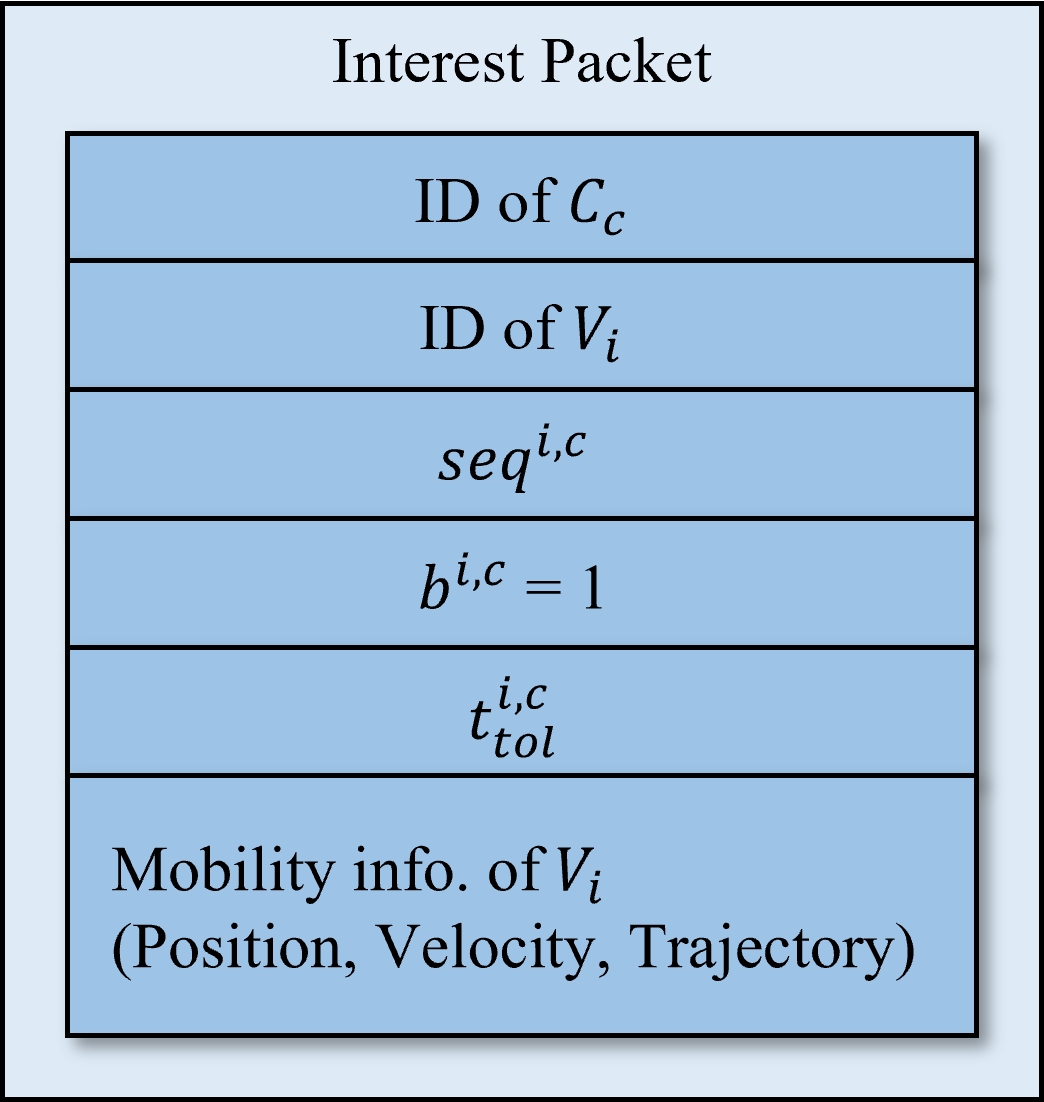
\includegraphics[width=0.23\textwidth]{./figure/Interest01.png}}
    \subfigure[]{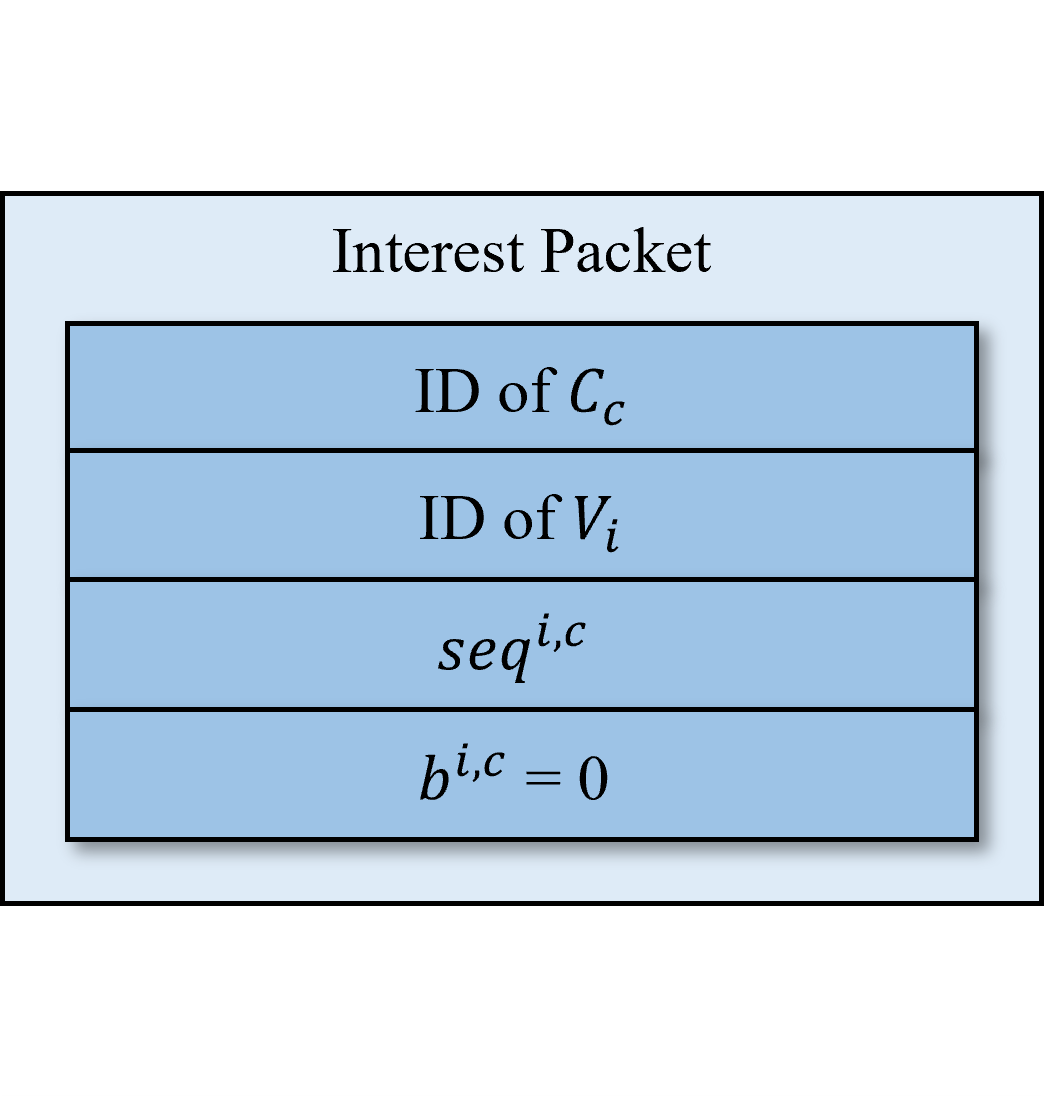
\includegraphics[width=0.23\textwidth]{./figure/Interest02.png}}
    \caption{The structure of $Interest$ packets (a) with $b^{i,c} = 1$; (b) with $b^{i,c} = 0$.}
    \label{fig:int}
\end{figure}

\begin{algorithm}
    \caption{$R_{j}$'s action with an $Interest$ packet.} \label{algo.int}
    \textbf{Input: } $Interest$ including $C_{c}$'s ID, $seq^{i,c}$, $b^{i,c}$, $t^{i,c}_{tol}$, and $V_{i}$'s info.(ID and mobility).\\
    \textbf{Output: } Action of $R_{j}$
    \begin{algorithmic}[1]
        \If {$b^{i,c} \neq 1$}
            \State $Data\{i, c, seq^{i,c}\}$ to $V_{i}$
        \Else
            \If {$!CS_{j}(c)$ and $t^{i,c}_{tol} > 0$ and $seq^{i,c} \neq 0$}
                \State $Deny\{i, c\}$ to $V_{i}$
                \State return
            \EndIf
            \State $Data\{i, c, seq^{i,c}\}$ to $V_{i}$
            \State $t^{i,j}_{dwell}$ Calculation
            \State $A_{ji} = t^{i,j}_{dwell} \times r_{j}(t)$
            \State $A_{remain} = (N_{c} - seq^{i,c}) \times s$
            \If {$t^{i,c}_{tol} > 0$ and $seq^{i,c} = 0$}
                \If {$A_{remain} > min(A_{ji}, t^{i,c}_{tol}\times r_{j}(t))$}
                    \State $Request$($Interest$) to content server of $C_{c}$
                \EndIf
            \EndIf
            \If {$t^{i,c}_{tol} = 0$ and $A_{remain} > A_{ji}$}
                \State $LastSeq = seq^{i,c} + Int(A_{ji} / s)$
                \State $Precaching(i'\text{s info.}, c, LastSeq)$ to $(j+1)$
            \EndIf
        \EndIf
    
    \end{algorithmic}
\end{algorithm}

When an RSU $R_{j}$ receives an $Interest$ packet from $V_{i}$, it follows the algorithm \ref{algo.int} to conduct its action.
In Lines 1 and 2, if $b^{i,c} \neq 1$, $R_{j}$ keeps providing $C_{c}$ to $V_{i}$ because it denotes that $R_{j}$ already decided to provide it.
Line 3 denotes that the decision is not made.
In Line 4, $CS_{j}(c)$ denotes the caching state of $R_{j}$' CS about $C_{c}$, which $CS_{j}(c)$ becomes the true value when the CS of $R_{j}$ stores $C_{c}$.
When the CS of $R_{j}$ doesn't have $C_{c}$, $CS_{j}(c)$ becomes the false value.
Lines 4--7 decide to send a $Deny$ packet to $V_{i}$ to prevent the participation of non-selected RSUs for the provision of the DTC, which is explained in subsection \ref{sec.p4}.
Otherwise, $R_{j}$ starts to provide $C_{c}$ to $V_{i}$.
Then, to know the size of the content that  $V_{i}$ can receive within the coverage of $R_{j}$, Line 9 calculates the dwell time $t^{i,j}_{dwell}$ of $V_{i}$ within $R_{j}$'s coverage based on euclidean distance calculation as follows:
\begin{equation}
    (p_{i}.x + tv_{i}.x - p_{j}.x)^{2}+(p_{i}.y + tv_{i}.y - p_{j}.y)^{2} = range^{2}_{j}, \label{eq:4}
\end{equation}
where $p_{i}.x$ and $p_{i}.y$ denotes the $x$-asix and $y$-asix position of $V_{i}$.
Also, $p_{j}.x$ and $p_{j}.y$ denotes the $x$-asix and $y$-asix position of $R_{j}$.
$v_{i}.x$ and $v_{i}.y$ denotes the $x$-asix and $y$-asix velocity of $V_{i}$.
$range_{j}$ denotes the communication range of $R_{j}$. 
Equation (\ref{eq:4}) can be rewritten as follows:\\
\begin{equation} \begin{split}
    & (v_{i}^{2}.x+v_{i}^{2}.y)t^{2}\\
    & + 2(v_{i}.x(p_{i}.x-p_{j}.x)+v_{i}.y(p_{i}.x-p_{i}.x))t \\
    & + ((p_{i}.x-p_{j}.x)^{2}+(p_{i}.y-p_{j}.y)^{2}-range^{2}_{j}) = 0. \label{eq:5}
\end{split} \end{equation}
To simplify the calculation, we can replace equation (\ref{eq:5}) with the following.\\
\begin{equation}
    Q_{1} = (v_{i}^{2}.x+v_{i}^{2}.y). \\
\end{equation}    
\begin{equation}
    Q_{2} = 2(v_{i}.x(p_{i}.x-p_{j}.x)+v_{i}.y(p_{i}.x-p_{i}.x)). \\
\end{equation}    
\begin{equation}
    Q_{3} = (p_{i}.y-p_{j}.y)^{2}-range^{2}_{j}). \\
\end{equation}
Because $V_{i}$ already enters within $R_{j}$'s coverage area, only a bigger value is taken between the two calculated values in the following equation (\ref{eq:9}) as $t^{i,j}_{dwell}$.
\begin{equation}
    t^{i,j}_{dwell} = \cfrac{-Q_{2}\pm\sqrt{Q_{2}^{2}-4Q_{1}Q_{3}}}{2Q_{1}}. \label{eq:9}
\end{equation}

Line 10 calculates the size of the content that $V_{i}$ can receive within the communication coverage of $R_{j}$.
To compare it, Line 11 calculates the remaining size of the content that $V_{i}$ has to receive.
Line 12 determines whether $C_{c}$ is DTC and it is the first $Interest$ packet from $V_{i}$ to download $C_{c}$.
Lines 13--15 send the $Request$ packet to the DMM when $C_{c}$ is DTC and it needs to be precached at sequential RSUs, where a $Request$ packet is explained in subsection \ref{sec.p2}.
In the case of DTC, when $R_{j}$ determines the need for precaching $C_{c}$, it considers the tolerable delay time $t^{i,c}_{tol}$ of $C_{c}$ as shown in Line 13.
For $C_{c}$ as DSC, line 17 determines to precache $C_{c}$ at the next RSU based on the mobility information of $V_{i}$ to minimize the delay for the provision of $C_{c}$.
Lines 18--20 send a $Precaching$ packet that includes the last chunk number $LastSeq$ of $C_{c}$ that $R_{j}$ can provide, where the $Precaching$ packet is explained in detail in subsection \ref{sec.p3}.
$Int(A_{ji} / s)$ represents the integerization of $A_{ji} / s$, which denotes the quotient of the calculation.



\subsection{Information Update Process} \label{sec.p2}
In order for DMM to be more effective in selecting the Optimal Precaching RSUs (OPRs) for DTC, it must optimize with predictions based on the latest information.
In this subsection, we thus explain the process to create the table of RSUs that are associated with providing $C_{c}$ to $V_{i}$ and updating the RSUs' information.
By improving the prediction accuracy of the selection based on the updated information, the performance of optimization in the DMM can be improved.
We assume that the processing delay for the update is very trivial in providing $C_{c}$ to $V_{i}$ because DTC $C_{c}$ has a tolerable delay time.
Furthermore, since the process only needs to be completed before $V_{i}$ enters the next RSU that is considered to become an OPR, it only needs to be completed while $V_{i}$ is receiving $C_{c}$ from the current RSU.
Through the short delay and the small traffic costs for the process, we can achieve the minimization of traffic consumption for DTC by reducing the movements of the bigger-sized $Data$ packet to provide DTC.

\begin{figure}
    \centering
    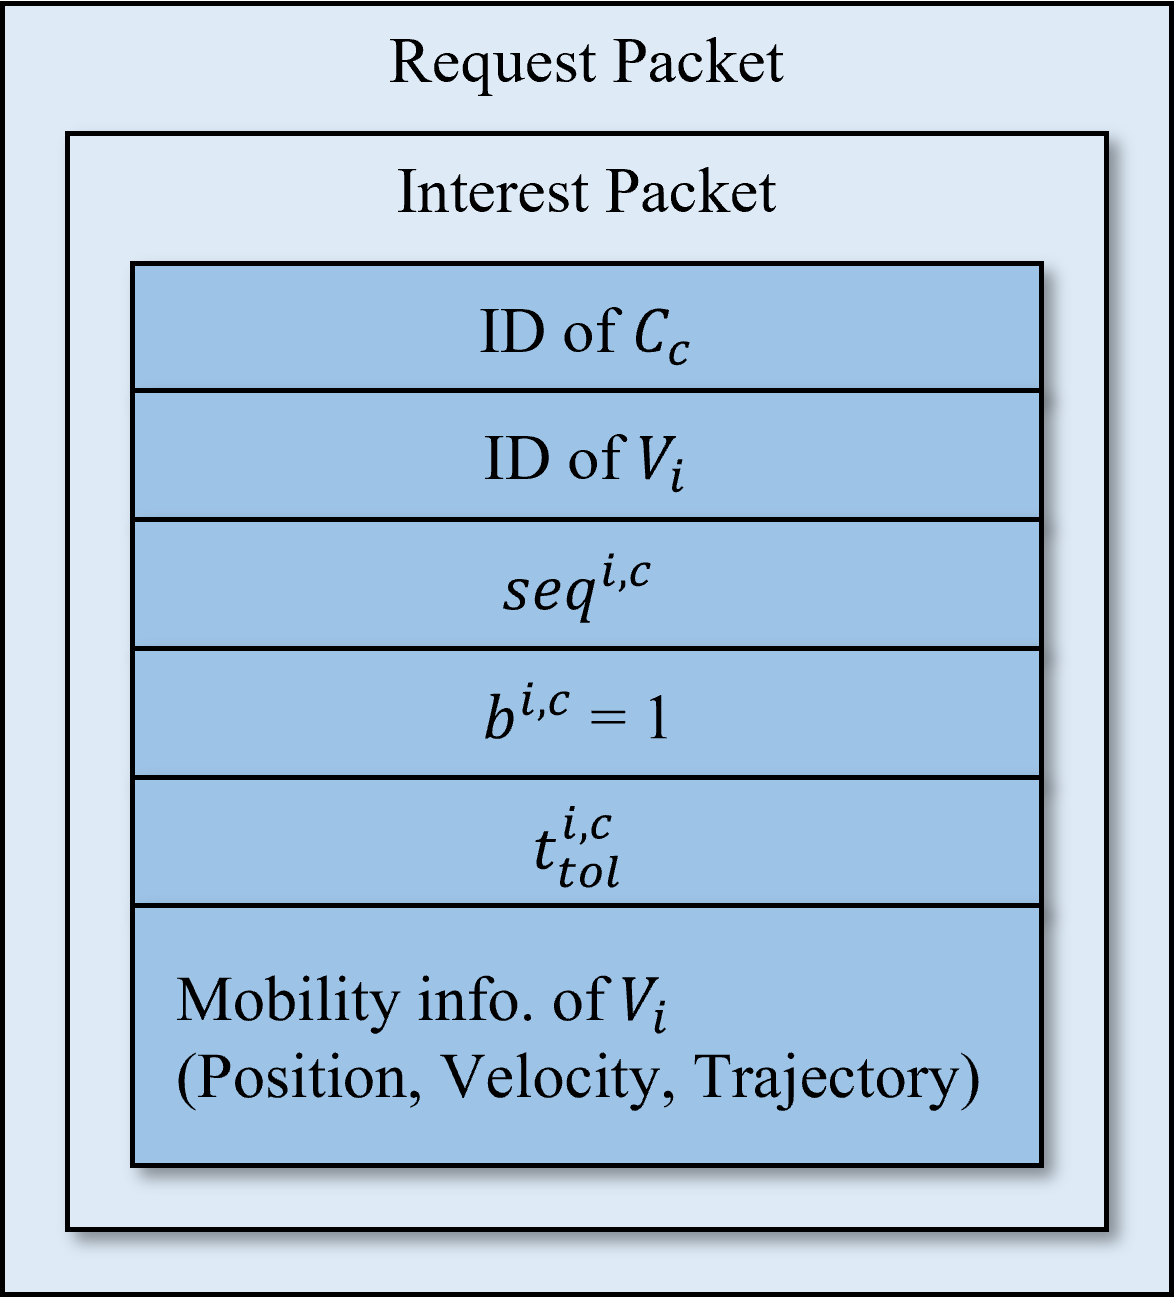
\includegraphics[width=0.23\textwidth]{./figure/Request.png}
    \caption{The structure of $Request$ packets.}
    \label{fig:req}
\end{figure}

To provide the necessary information to solve an ILP optimization of selecting OPRs to the DMM, RSUs include an $Interest$ packet in a $Request$ packet because the $Interest$ packet already contains the necessary information.
Since the $Request$ packet contains the $Interest$ packet with $b^{i,c}=1$, it is designed with the same structure as shown in Fig. \ref{fig:req}.
When an intermediate RSU receives the $Request$ packet, it further forwards the packet to the content server of $C_{c}$ that is contained in the packet.
When the content server receives the $Request$ packet, it moves the packet to its DMM.
To select OPRs, the DMM creates a candidates table.
Based on $V_{i}$'s mobility information and $t^{i,c}_{tol}$ contained in the packet, the DMM defines the precaching available area $PAA^{i,c}$, which is the area to be able to precache $C_{c}$ for providing $C_{c}$ to $V_{i}$.
First, by using the position and trajectory information of $V_{i}$, the DMM draws the trajectory area that $V_{i}$ will travel in the map that the DMM has.
Then, using $V_{i}$'s velocity and $t^{i,c}_{tol}$, it defines $PAA^{i,c}$ as the trajectory between the current position of $V_{i}$ and the reachable position that $V_{i}$ can reach within $t^{i,c}_{tol}$ on the entire trajectory.
The DMM stores the ID of every RSU in $PAA^{i,c}$ in a candidates table for providing $C_{c}$ to $V_{i}$ as $PAR^{i,c}_{k}$, where $PAR^{i,c}_{k}$ is the $k$-th RSU in the order in which $V_{i}$ will encounter in $PAA^{i,c}$.

\begin{figure}
    \centering
    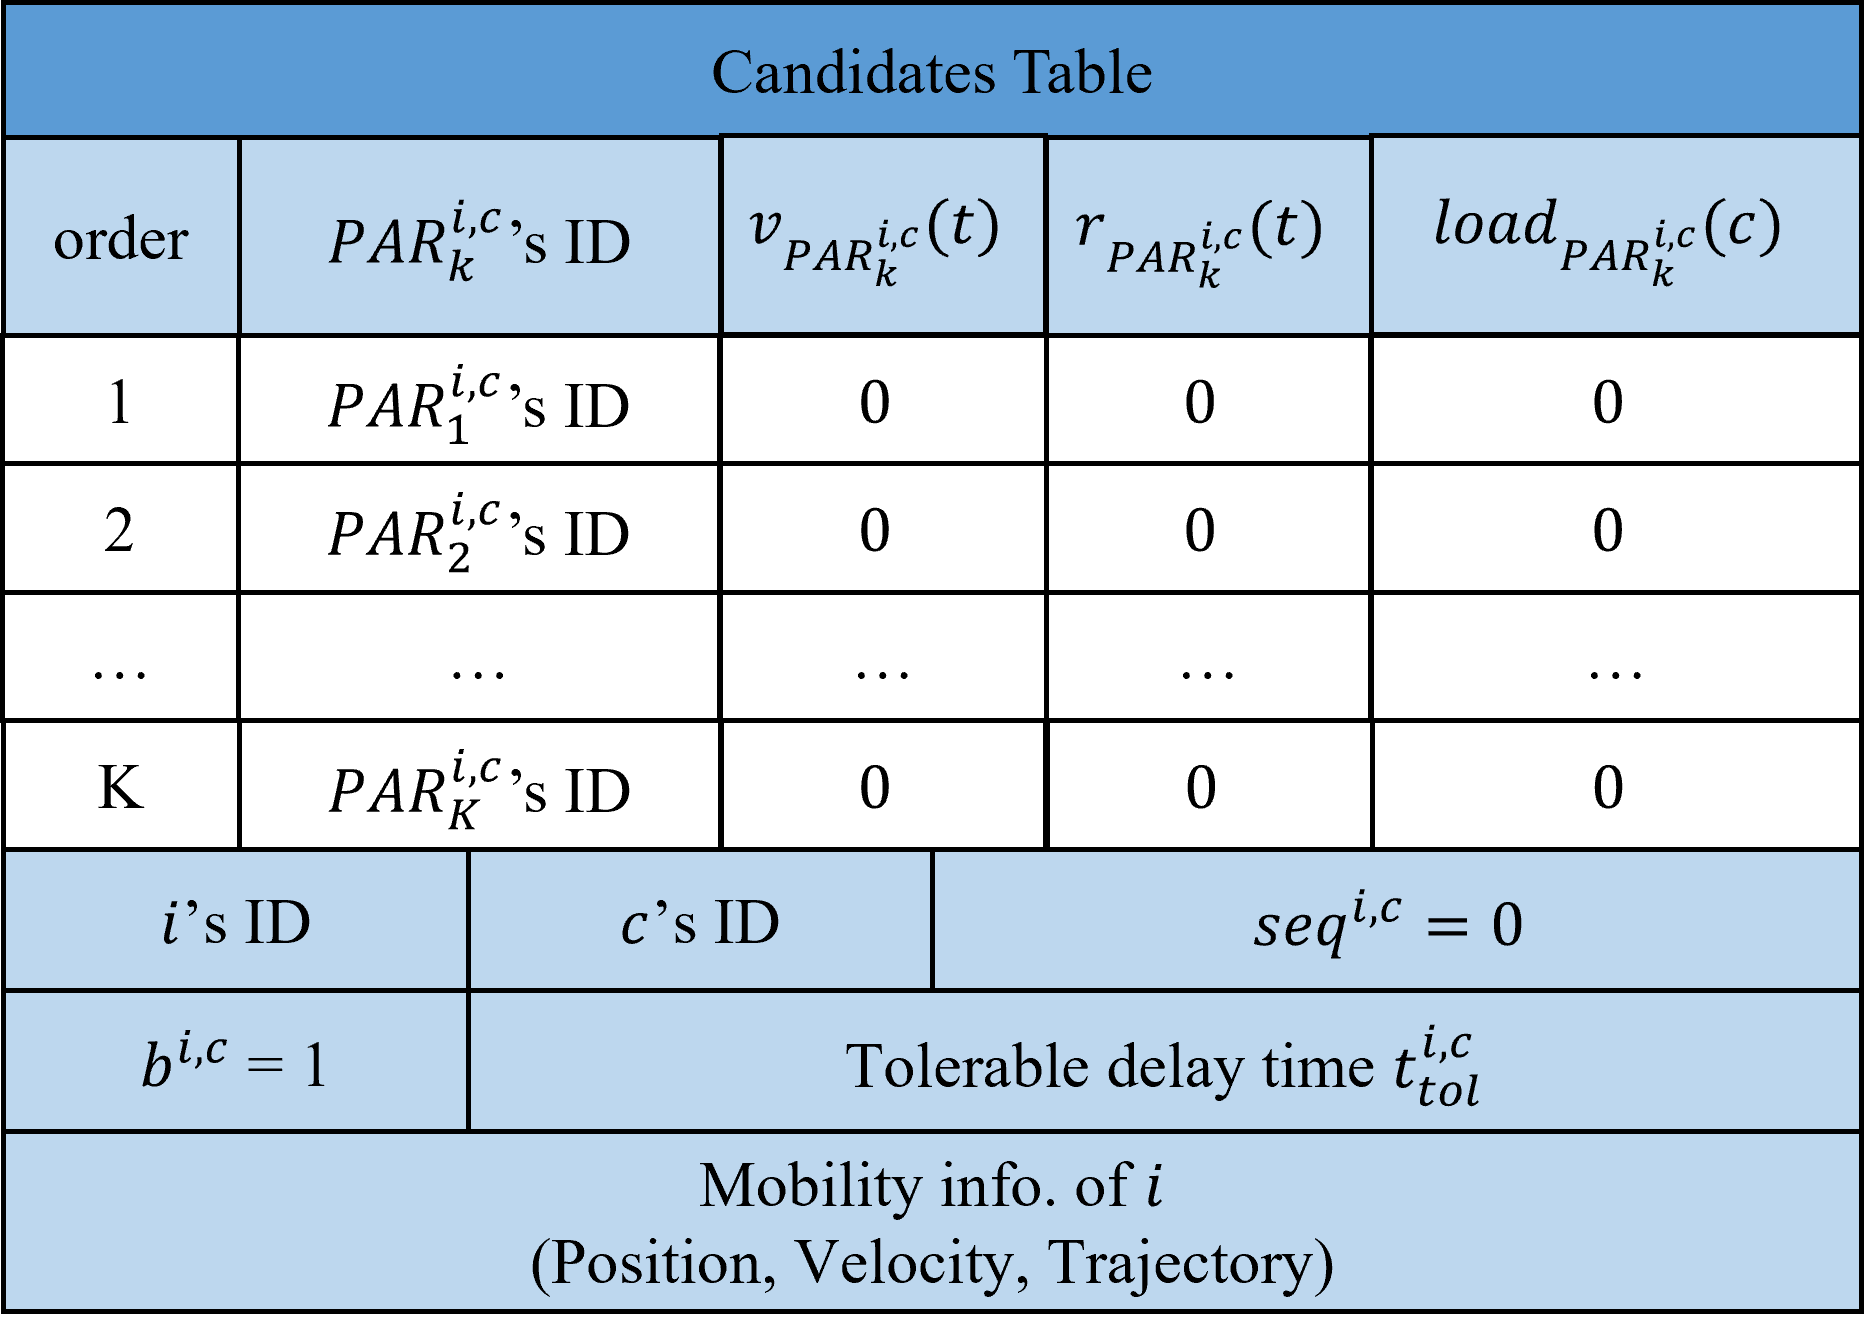
\includegraphics[width=0.4\textwidth]{./figure/ctable01.png}
    \caption{The structure of the candidates table created for the provision of $C_{c}$ to $V_{i}$ in the DMM.}
    \label{fig.ctable1}
\end{figure}

When the DMM creates a candidate table, it initializes the candidates table as shown in Fig. \ref{fig.ctable1}.
$r_{PAR^{i,c}_{k}}(t)$ denotes the average transmission rate of $PAR^{i,c}_{k}$.
$load_{PAR^{i,c}_{k}}(c)$ denotes the burden value to ready $C_{c}$ in the CS of $PAR^{i,c}_{k}$, which is explained later.
Since the DMM does not have any information about $PAR^{i,c}_{k}$ at this time, all of $v_{PAR^{i,c}_{k}}(t)$, $r_{PAR^{i,c}_{k}}(t)$, and $load_{PAR^{i,c}_{k}}(c)$ are initialized as 0.
To solve the optimization problem later, the information that is contained in the $Request$ packet is stored in the table.
To update the latest information, the DMM sends the $Information$ $Request$ packet to each $PAR^{i,c}_{k}$, where the packet contains the ID of each $PAR^{i,c}_{k}$ and the ID of $C_{c}$.


\begin{algorithm}
    \caption{$R_{j}$'s action with an $Information$ $Request$ packet.} \label{algo.req}
    \textbf{Input: } $InfoReq$ including $C_{c}$'s ID and $PAR^{i,c}_{k}$'s ID.\\
    \textbf{Output: } Action of $R_{j}$.
    \begin{algorithmic}[1]
        \If {$ID_{j} \neq ID_{PAR^{i,c}_{k}}$}
            \State Forwarding the packet to the next RSU
        \Else
            \If {$CS_{j}(c)$}
                \State $InfoRep(c, ID_{j}, v_{j}(t), r_{j}(t), 0)$ to the server
                \State $Update\_CS_{j}(c)$
            \Else
                \State $ID_{next}$ = FIB($C_{c}$)
                \State $InstInt(ID_{j}, ID_{PAR^{i,c}_{k}}, c)$ to $ID_{next}$
                \State Instant PIT \textleftarrow $InstInt(ID_{j}, ID_{PAR^{i,c}_{k}}, c)$
            \EndIf
        \EndIf
    \end{algorithmic}
\end{algorithm}

The RSU $R_{j}$ follows the algorithm \ref{algo.req} for its action when it receives the $Information$ $Request$ packet, which is designed as shown in Fig. \ref{fig:Info}(a).
Lines 1 and 2 represent the forwarding of the packet to the next RSU if its ID is different from the ID that is contained in the packet.
Line 3 indicates that the packet reaches $PAR^{i,c}_{k}$.
Lines 4 and 5 describe sending the necessary information through the $Information$ $Reply$ packet in Fig. \ref{fig:Info}(b) to the content server of $C_{c}$ if this $PAR^{i,c}_{k}$ is $ACR^{i,c}_{k}$ because it already caches $C_{c}$ in its CS.
In this case, since it doesn't need to consume additional traffic to bring $C_{c}$ into its CS, $PAR^{i,c}_{k}$ puts $load_{PAR^{i,c}_{k}}(c)$ as 0 into the $Information$ $Reply$ packet.
Also, Line 6 updates the priority of $C_{c}$ to prevent it from being replaced by other contents due to storage limitations.
Line 7 indicates that $PAR^{i,c}_{k}$ is $NCR^{i,c}_{k}$ because it does not have $C_{c}$ in its CS.
In Lines 8 and 9, this $NCR^{i,c}_{k}$ sends the $Instant$ $Interest$ packet to the next RSU based on its FIB.
Then, Line 10 stores the $Instant$ $Interest$ packet in the instant PIT, which has the same structure as the PIT.

\begin{figure}
    \centering
    \subfigure[]{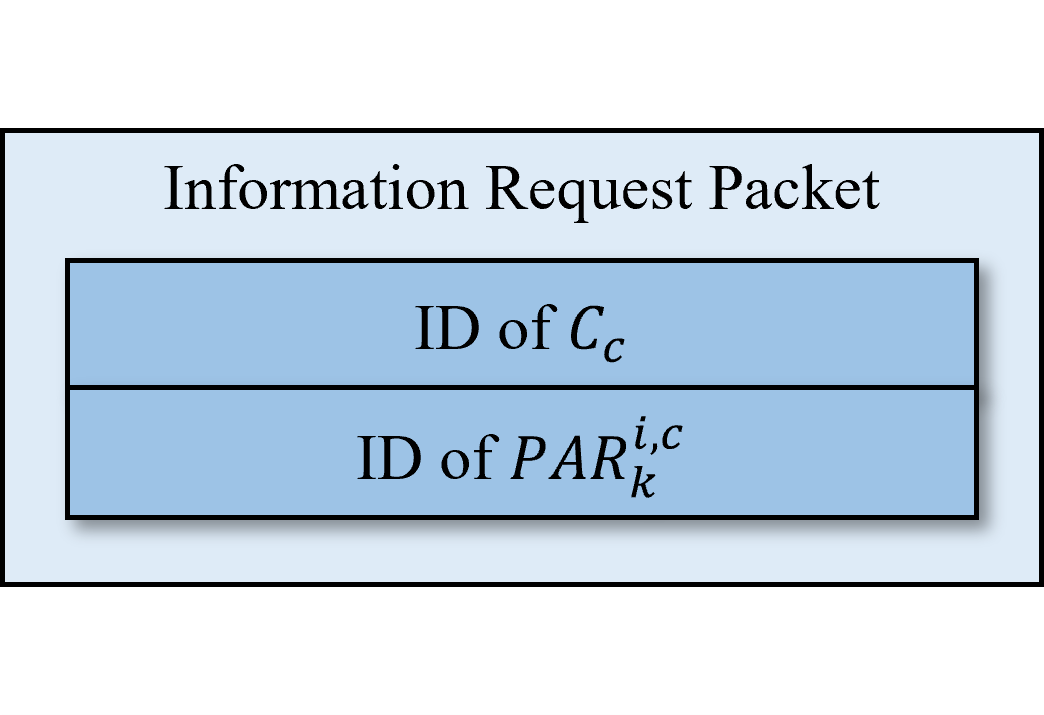
\includegraphics[width=0.23\textwidth]{./figure/InfoReq.png}}
    \subfigure[]{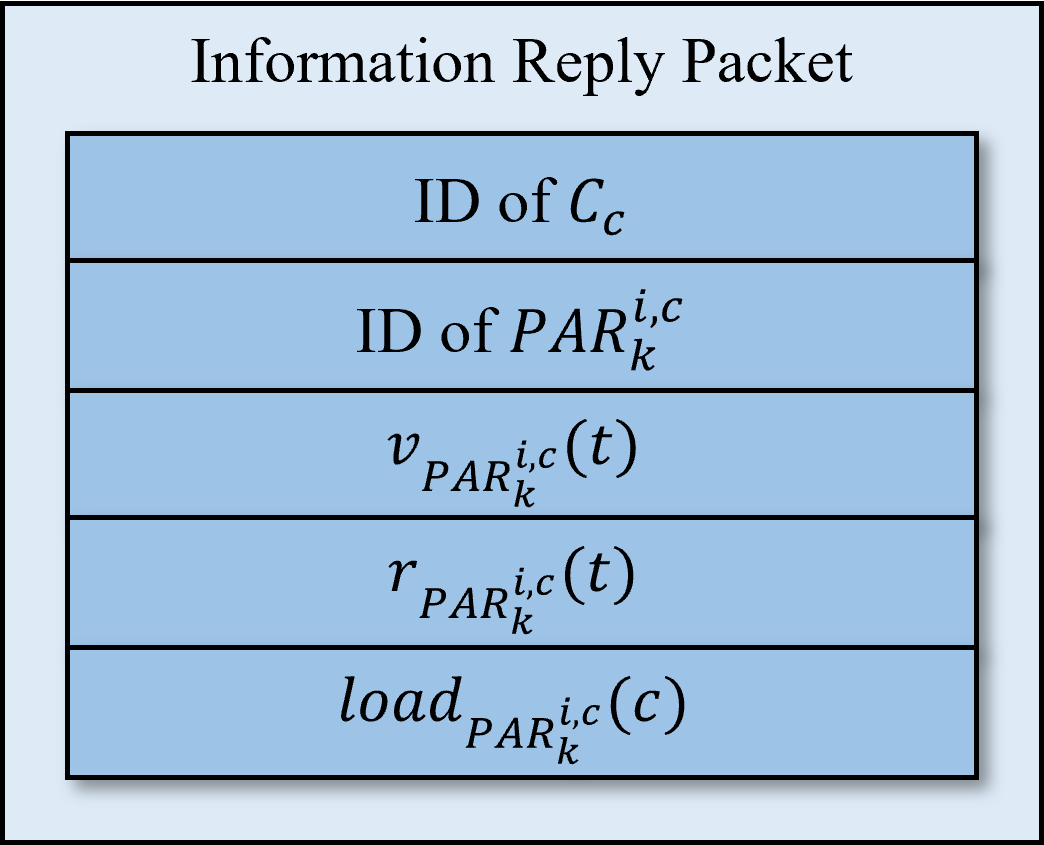
\includegraphics[width=0.23\textwidth]{./figure/InfoRep.png}}
    \caption{The structure of (a) $Information$ $Request$ packets; (b) $Information$ $Reply$ packets.}
    \label{fig:Info}
\end{figure}


\begin{figure}
    \centering
    \subfigure[]{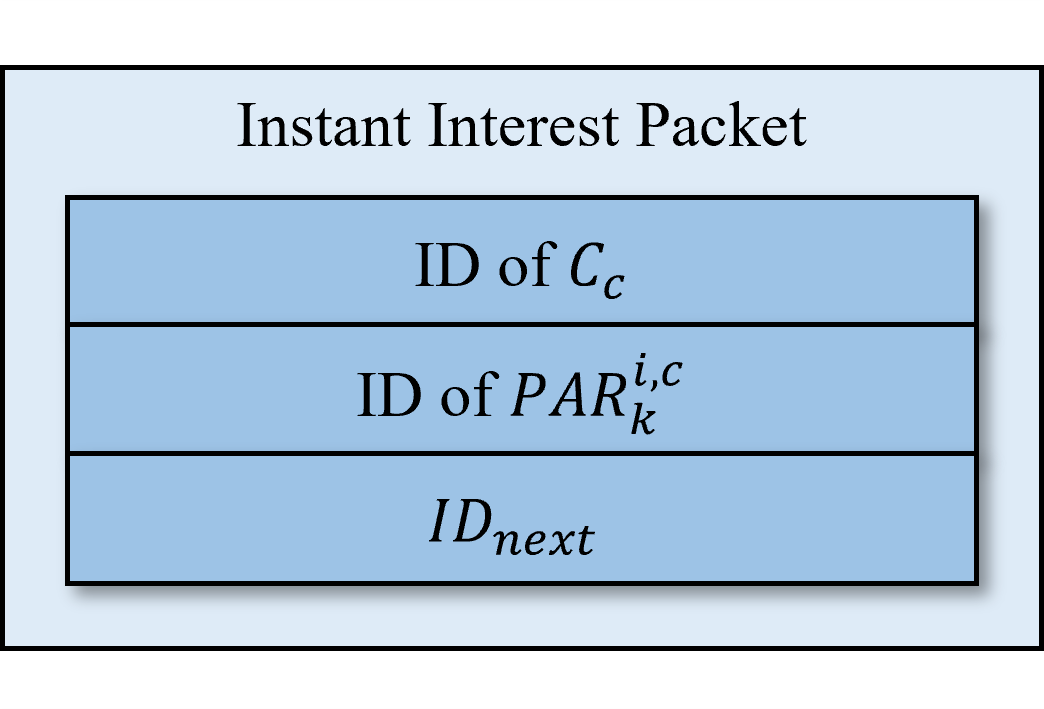
\includegraphics[width=0.23\textwidth]{./figure/InstInt.png}}
    \subfigure[]{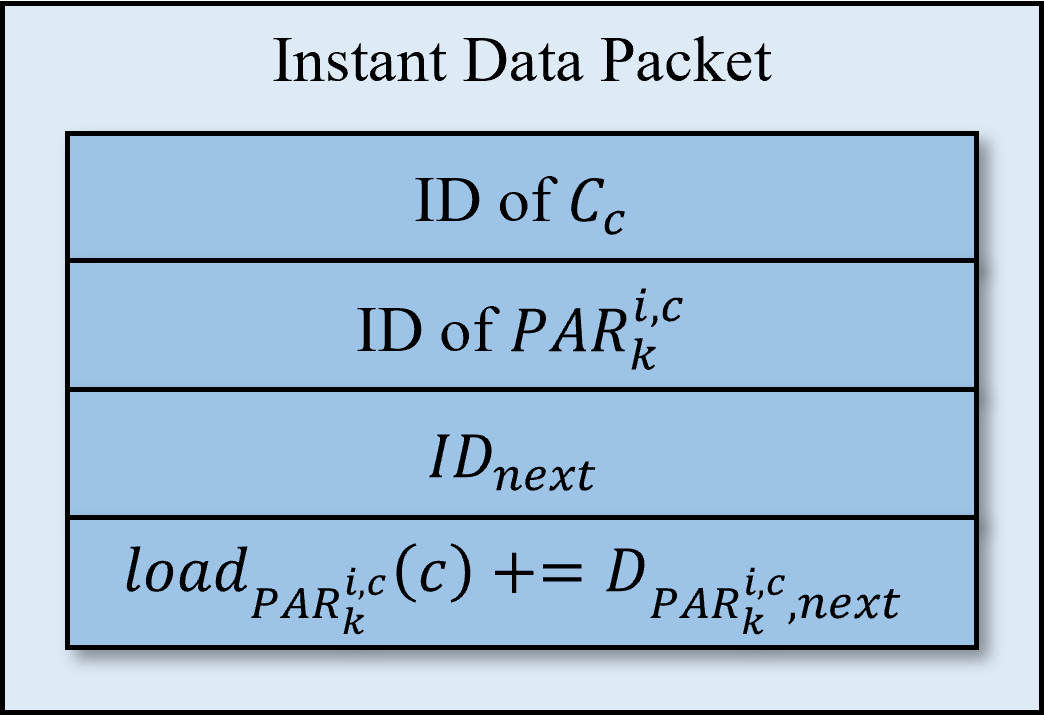
\includegraphics[width=0.23\textwidth]{./figure/InstData.png}}
    \caption{The structure of (a) $Instant$ $Interest$ packets; (b) $Instant$ $Data$ packets.}
    \label{fig:inst}
\end{figure}

If an RSU that receives an $Instant$ $Interest$ packet doesn't have $C_{c}$ in its CS, it stores the packet in its instant PIT and forwards the packet to the next RSU based on its FIB.
Fig. \ref{fig:inst}(a) shows the structure of $Instant$ $Interest$ packet. 
The forwarded $Instant$ $Interest$ packet includes the next RSU's ID, the saved $NCR^{i,c}_{k}$'s ID, and $C_{c}$'s ID.
If the $Instant$ $Interest$ packet arrives at the provider of $C_{c}$, which can be an RSU or the content server, the provider sends the $Instant$ $Data$ packet to the saved previous RSU's ID, where the packet includes the saved $NCR^{i,c}_{k}$'s ID, $C_{c}$'s ID, and the initialized $load_{NCR^{i,c}_{k}}(c)$.
Then, the $Instant$ $Data$ packet is designed as shown in Fig. \ref{fig:inst}(b).
Since this $Instant$ $Data$ packet does not contain any chunks of $C_{c}$, its size is very small.
The first $load_{NCR^{i,c}_{k}}(c)$ is initialized as the burden value to use the link between the provider and the previous RSU.
To calculate the burden value $D_{m,(m-1)}(t)$, which is the burden value to use the link between the provider $R_{m}$ and the previous RSU $R_{(m-1)}$, the average link usage $U_{m,(m-1)}(t)$ between $R_{m}$ and $R_{(m-1)}$ has to be obtained.
As a ratio of the consumed traffic to the total link capacity, $U_{m,(m-1)}(t)$ is also obtained through the same equation with the given Eq. \ref{eq1} as follows:
\begin{equation}
    U_{m,(m-1)}(t) = \cfrac{\sum_{q=0}^{t_{max}}U_{m,(m-1)}(t-q)}{t_{max}}.    \label{eq3}
\end{equation}
As a router, $R_{m}$ monitors the link capacity, traffic usage, etc. for each port and statistically averages each of them at each time $t$.
Since $U_{m,(m-1)}(t)$ is the ratio of the usage, it can be a value between 0 and 1.
Also, $U_{m,(m-1)}(t)$ is also updated by $t_{max}$.
By using $U_{m,(m-1)}(t)$, $D_{m,(m-1)}(t)$ is defined as follows:
\begin{equation}
    D_{m,(m-1)}(t) = \cfrac{1}{1-U_{m,(m-1)}(t)}.
\end{equation}
Thus, if the link is used 100 $\%$, $D_{m,(m-1)}(t)$ becomes the infinite.

When intermediate RSUs receive the $Instant$ $Data$ packet, it searches the element consisting of the saved $NCR^{i,c}_{k}$'s ID and $C_{c}$'s ID in its instant PIT.
Based on the previous RSU's ID of the matched element, the intermediate RSUs forward the $Instant$ $Data$ packet to the ID, where $load_{NCR^{i,c}_{k}}(c)$ in the packet is updated by adding $D_{m,(m-1)}(t)$.
Then, the RSUs erase the $Instant$ $Data$ packet in its instant PIT.
Therefore, in the process of forwarding the $Instant$ $Data$ packet, each intermediate RSU keeps adding its $D_{m,(m-1)}(t)$ to $load_{NCR^{i,c}_{k}}(c)$.
When an RSU receives this packet, it can notice whether the RSU is $NCR^{i,c}_{k}$ because the packet contains the ID of $NCR^{i,c}_{k}$.
Since the packet already has the completed $load_{NCR^{i,c}_{k}}(c)$ via the intermediate RSUs, $NCR^{i,c}_{k}$ sends the $Information$ $Reply$ packet to the content server of $C_{c}$, where the packet contains $C_{c}$'s ID, $NCR^{i,c}_{k}$'s ID, $v_{NCR^{i,c}_{k}}(t)$, $r_{NCR^{i,c}_{k}}(t)$, and completed $load_{NCR^{i,c}_{k}}(c)$ as shown in Fig. \ref{fig:Info}(b).



\subsection{Selection of Optimal Precaching RSU} \label{sec.p3}
In the case that $C_{c}$ is DTC, to minimize the traffic consumption for the provision of $C_{c}$ within $t^{i,c}_{tol}$, the optimization for the selection of $OPR^{i,c}_{k}$ minimizes the movement of the $Data$ packet for consuming to provide or precache $C_{c}$ to $V_{i}$ by using as many $ACR^{i,c}_{k}$ as possible that already caches $C_{c}$ in their own CS.
Also, because the DMM takes $t^{i,c}_{tol}$ into the optimization, it can guarantee high reliability in providing $C_{c}$ to $V_{i}$ within $t^{i,c}_{tol}$.
Additionally, considering the opportunity cost of holding $C_{c}$ in the CS of $ACR^{i,c}_{k}$ until $V_{i}$ enters the coverage area of $ACR^{i,c}_{k}$, the caching burden is minimized by preparing $C_{c}$ in the nearest $ACR^{i,c}_{k}$.
Furthermore, if it is necessary to use $NCR^{i,c}_{k}$ to precache $C_{c}$, the traffic concentration is minimized by selecting the most free $NCR^{i,c}_{k}$ on the link.
To solve an optimization problem that achieves this goal, the DMM must decide whether $NCR^{i,c}_{k}$ needs to be used based on the amount of $C_{c}$ provided to $V_{i}$ by $ACR^{i,c}_{k}$ or not.
Also, to know how many $NCR^{i,c}_{k}$ should precache $C_{c}$, we need to calculate the amount of $C_{c}$ that each $NCR^{i,c}_{k}$ can provide to $V_{i}$.
Therefore, we first calculate the amount of $C_{c}$ that each $PAR^{i,c}_{k}$ can provide to $V_{i}$.
In this subsection, we solve the optimization problem to reach the goal based on the calculated and updated information.

As mentioned in the previous subsection, the DMM receives an $Information$ $Reply$ packet for $C_{c}$ from an RSU.
Based on the received $Information$ $Reply$ packet, the DMM finds all the candidates tables for $C_{c}$ in it and updates the information of $PAR^{i,c}_{k}$'s ID included in the packet in those tables.
When the information of all $PAR^{i,c}_{k}$ in the candidates table is updated, the DMM solves an optimization problem to minimize the traffic consumption for providing the DTC $C_{c}$ to $V_{i}$, based on the information in the stored $Request$ packet and the information in the candidate table.
To do this, it must first calculate the amount of $C_{c}$ that can be provided to $V_{i}$ from each $PAR^{i,c}_{k}$, because $V_{i}$ has only a limited time to stay at each $PAR^{i,c}_{k}$.
For providing $C_{c}$ to $V_{i}$, the amount $A_{down}^{i, 1}(c)$ of $C_{c}$ that can be provided to $V_{i}$ by the first $PAR^{i,c}_{k}$ (i.e. $PAR^{i,c}_{1}$)  is calculated as follows:
\begin{equation} % eq1
    \begin{split}
        & A_{down}^{i, 1}(c)\\ & = \begin{cases*}
            t_{dwell}^{i, PAR^{i,c}_{1}} \times r_{PAR^{i,c}_{1}}, \text{if $PAR^{i,c}_{1}=ACR^{i,c}_{1}$},\\
            t_{dwell}^{i, PAR^{i,c}_{1}} \times \left(r_{PAR^{i,c}_{1}}^{-1}+ l^{-1} \right), else,
        \end{cases*} \label{eq:b}
    \end{split}
\end{equation}
where $t_{dwell}^{i, PAR^{i,c}_{1}}$ is the dwell time of $V_{i}$ within the coverage of $PAR^{i,c}_{1}$, which is calculated by the average speed $v_{PAR^{i,c}_{1}}(t)$ of vehicles within the coverage of $PAR^{i,c}_{1}$ and the coverage range of $PAR^{i,c}_{1}$.
The first chunk number considered in the optimization problem is calculated by $seq_{start}^{i,c}=1+Int(A_{down}^{i, 1}(c)/s)$, which represents the number of chunks that $PAR^{i,c}_{1}$ can provide to $V_{i}$.
$s$ is the size of one chunk and $Int()$ function denotes the quotient of the calculation.
From $PAR^{i,c}_{2}$ onward, every $PAR^{i,c}_{k}$ only cares about its own transmission rate $r_{PAR^{i,c}_{k}}$, since it precaches and prepares $C_{c}$.
However, since $t^{i,c}_{tol}$ limits the number of RSUs that $V_{i}$ will enter and does not make the last $PAR^{i,c}_{K}$ use the entire proportion of its dwell time $t^{i,PAR^{i,c}_{K}}_{dwell}$ to provide $C_{c}$ to $V_{i}$, we have to know the time that each $PAR^{i,c}_{k}$ can provide $C_{c}$ to $V_{i}$ within $t^{i,c}_{tol}$ based on the entrance time of $V_{i}$ into $PAR^{i,c}_{k}$.
As the definition of $PAA^{i,c}$, the DMM uses the trajectory of $V_{i}$ with the map to know the entrance time $t_{ent}^{i, PAR^{i,c}_{k}}$ during $t_{tol}^{i,c}$.
Therefore, the downloadable time $t_{down}^{i, PAR^{i,c}_{k}}$, which is the time to download $C_{c}$ from $PAR^{i,c}_{k}$, can be calculated by $t_{tol}^{i,c}-t_{ent}^{i, (j+K)}$.
Then, from $PAR^{i,c}_{2}$ onward, the providable amount of $C_{c}$ that $V_{i}$ can receive from ${PAR^{i,c}_{1}}$ can be calculated as follows:
\begin{equation}
    A_{prov}^{i, k}(c) = \begin{cases*}
        t_{down}^{i, PAR^{i,c}_{K}} \times r_{j+K}, & if $k=K$,\\
        t_{dwell}^{i, PAR^{i,c}_{k}} \times r_{j+k}, & else.\\
    \end{cases*} \label{eq:c}
\end{equation}


Based on $A_{prov}^{i, k}(c)$ and $seq_{start}^{i,c}$, the DMM selects $OPR^{i,c}_{k}$ to minimize the traffic consumption in the provision of $C_{c}$ to $V_{i}$ within $t_{tol}^{i,c}$.
The objective function has to minimize the traffic consumption by preferentially selecting $ACR^{i,c}_{k}$ with $load_{ACR^{i,c}_{k}}(c)$ of 0.
Then, to minimize the caching burden, it has to select $ACR^{i,c}_{k}$ that $V_{i}$ can reach as quickly as possible.
If the total $A_{prov}^{i, k}(c)$ of $ACR^{i,c}_{k}$ is not sufficient to complete providing $C_{c}$ to $V_{i}$ within $t_{tol}^{i,c}$, it has to consider $NCR^{i,c}_{k}$ as $OPR^{i,c}_{k}$.
In the selection of $OPR^{i,c}_{k}$ among $NCR^{i,c}_{k}$, it has to consider $load_{NCR^{i,c}_{k}}(c)$ to minimize the traffic concentration.
Also, to consider the caching burden of $ACR^{i,c}_{k}$ to hold $C_{c}$ until $V_{i}$ enters, we normalize it to a value between 0 and 1 by using $t_{ent}^{i, PAR^{i,c}_{k}}$ and $t^{i,c}_{tol}$.
Thus, to consider the caching burden of $ACR^{i,c}_{k}$ and $load_{NCR^{i,c}_{k}}(c)$ of $NCR^{i,c}_{k}$, we denote the total burden $Bd^{i,c}_{k}$ for preparing $c$ at every $OPR^{i,c}_{k}$ as follows:
\begin{equation}
    \begin{split}
        &Bd^{i,c}_{k}\\ &= \begin{cases*}
            t_{ent}^{i, PAR^{i,c}_{k}}/t^{i,c}_{tol}, & if $PAR^{i,c}_{k}=ACR^{i,c}_{k}$,\\
            1 + load_{PAR^{i,c}_{k}}(c), & else.\\
        \end{cases*} 
    \end{split}\label{eq:d}
\end{equation}
For considering the caching burden of $ACR^{i,c}_{k}$ to hold $C_{c}$ until $V_{i}$ enters, we normalize it to a value between 0 and 1 by using $t_{ent}^{i, PAR^{i,c}_{k}}$ and $t^{i,c}_{tol}$.
Since the caching burden is less than 1, $ACR^{i,c}_{k}$ has a higher priority to become $OPR^{i,c}_{k}$ because we add 1 to $load_{NCR^{i,c}_{k}}(c)$ of $NCR^{i,c}_{k}$ in the Eq. (\ref{eq:d}).
Accordingly, if $C_{c}$ is DTC, the optimization problem is defined as follows in order to minimize the burden to provide $C_{c}$ to $V_{i}$ in the case that $PAR^{i,c}_{1}$ can not complete providing $C_{c}$ to $V_{i}$ within $t_{dwell}^{i,PAR^{i,c}_{1}}$.
\begin{align}
    min\quad &  o^{i,c} = \sum_{k=2}^{K}Bd^{i,c}_{k}\sum_{n=seq_{start}^{i,c}}^{N_{c}} \xi^{i,k}(h_{n}^{c})\\
    \text{s.t.} \quad & \sum_{k=2}^{K} \xi^{i, k}(h_{n}^{c}) = 1 \\
    & \sum_{k=2}^{K}\sum_{n=seq_{start}^{i,c}}^{N_{c}} \xi^{i, k}(h_{n}^{c}) = (N_{c}-seq_{start}^{i,c})\\
    & \sum_{n=seq_{start}^{i,c}}^{N_{c}} s\times\xi^{i, k}(h_{n}^{c}) \leq A_{prov}^{i, k}(c)\\
    & \xi^{i,k}(h_{n}^{c}) \in \{0, 1\} \\
    & load_{PAR^{i,c}_{k}}(c)\geq 1,
\end{align}
where $\xi^{i,k}(h_{n}^{c})$ indicates whether $OPR^{i,c}_{k}$ precaches the $n$-th chunk $h_{n}^{c}$ of $C_{c}$ for providing it to $V_{i}$.
If $OPR^{i,c}_{k}$ precaches  $h_{n}^{c}$ in its CS, $\xi^{i,k}(h_{n}^{c})$ is 1.
Otherwise, $\xi^{i,k}(h_{n}^{c})$ is 0.
The objective function denotes the total burden to precache each chunk $h_{n}^{c}$ at the CS of $OPR^{i,c}_{k}$.
Thus, it can minimize the sum of the caching burden and $load_{OPR^{i,c}_{k}}(c)$ that contains the link usage burden.
As a result, the traffic consumption, the traffic concentration, and the caching burden can be minimized.
To solve this optimization problem, we set several constraints.
The constraint of the equation (16) prevents the precached chunk from being precached in the CS of other $OPR^{i,c}_{k}$ because only one chunk can be precached in the CS of all $OPR^{i,c}_{k}(c)$.
This can also prevent redundant precaching.
The constraint of equation (17) makes the total number of the precaching chunks equal to the number of chunks that should be provided to $V_{i}$ because it can omit some chunks.
The constraint of the equation (18) limits the precachable number of chunks to $A_{prov}^{i, k}(c)$ because it can precache all chunks in the CS of the nearest $ACR^{i,c}_{k}$.
The constraint of equation (19) indicates the characteristic of $\xi^{i,k}(h_{n}^{c})$ and the constraint of equation (20) indicates the characteristic of $load_{OPR^{i,c}_{k}}(c)$, respectively.
After obtaining $\xi^{i,k}(h_{n}^{c})$ through the optimization, the DMM decides the start and the last numbers of chunks that each $OPR^{i,c}_{k}$ has to precache.
The start chunk number $seq_{min}^{i,c}$ to be precached in the CS of $OPR^{i,c}_{k}$ is denoted as follows: 
\begin{equation}
    seq_{min}^{i,c} = seq^{i,c}_{start}+\sum_{q=2}^{k-1} \xi^{i,q}(h_{n}^{c})+1.
\end{equation}
Also, the last chunk number $seq_{max}^{i,c}$ to be precached in the CS of $OPR^{i,c}_{k}$ is denoted as follows:
\begin{equation}
    seq_{max}^{i,c} = seq^{i,c}_{start}+\sum_{q=2}^{k} \xi^{i,q}(h_{n}^{c}).
\end{equation}
The DMM then sends a $Precaching$ packet, which is designed as shown in Fig. \ref{fig:prec}.
After sending it, the DMM erases the candidates table for DTC $C_{c}$.

\subsection{Provision of the requested content} \label{sec.p4}
In this subsection, we describe how TOCP achieves the provision of a requested content $C_{c}$ to $V_{i}$ through RSUs.
If an RSU receives a $Precaching$ packet for $C_{c}$, it prepares the chunks of $C_{c}$ based on the received $Precaching$ packet.
The RSU can distinguish whether the $Precaching$ packet is for DSC or DTC based on the information contained in the $Precaching$ packet.
Then, TOCP can minimize the access delay for DSC and guarantee reliability for DTC.
Also, since only $OPR^{i,c}_{k}$ participates in providing DTC to $V_{i}$, TOCP can minimize the traffic consumption.

\begin{figure}
    \centering
    \subfigure[]{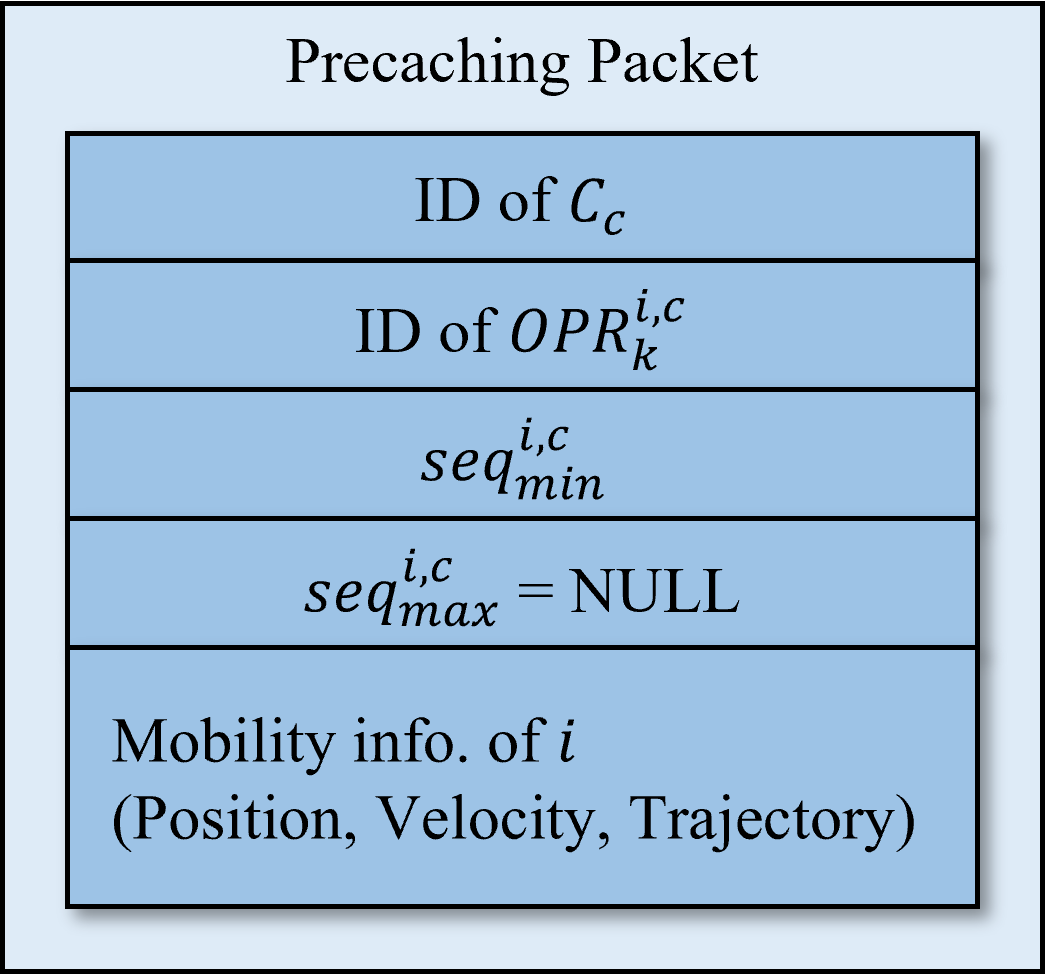
\includegraphics[width=0.23\textwidth]{./figure/Precaching01.png}}
    \subfigure[]{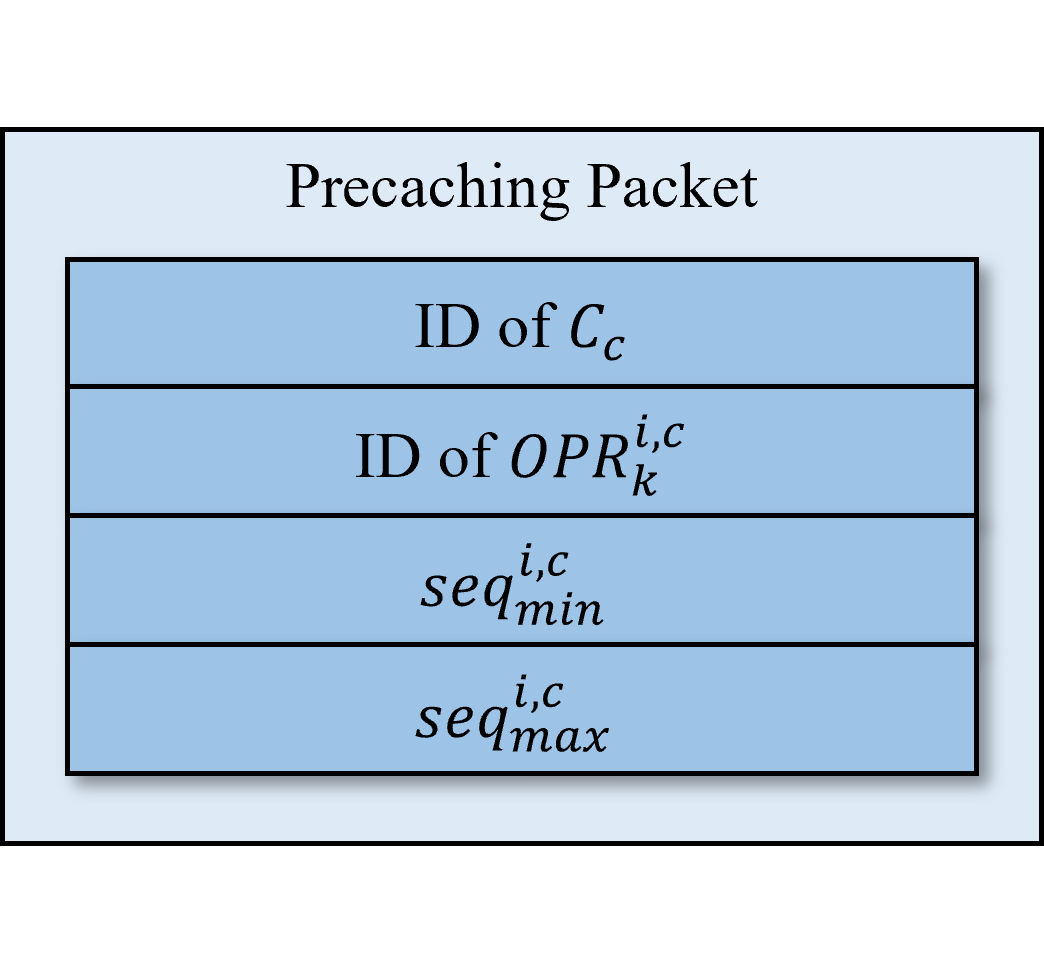
\includegraphics[width=0.23\textwidth]{./figure/Precaching02.png}}
    \caption{The structure of $Precaching$ packets (a) without $seq^{i,c}_{max}$; (b) with $seq^{i,c}_{max}$.}
    \label{fig:prec}
\end{figure}


When a $Precaching$ packet arrives $OPR^{i,c}_{k}$ which has the same ID as the ID contained in the packet, $OPR^{i,c}_{k}$ checks $seq^{i,c}_{max}$ to know whether the packet comes from a previous RSU for precaching DSC or from the DMM for preparing DTC.
Fig. \ref{fig:prec} shows the structure of $Precaching$ packets designed in TOCP.
Fig. \ref{fig:prec}(a) represents the $Precaching$ packet received from the previous RSU to minimize the access delay in providing DSC.
In this case, since the RSU that receives the $Precaching$ packet calculates the providable amount of the content and precaches the providable number of the chunks, the packet contains the last chunk number that the previous RSU can provide and the mobility information of the requester vehicle $V_{i}$.
Fig. \ref{fig:prec}(b) represents the $Precaching$ packet received from the DMM.
In this case, since the providable number of the chunks is already calculated by the DMM, the $Precaching$ packet doesn't have to contain the mobility information of the requester vehicle $V_{i}$.
Also, the RSU that receives this packet has to ready the chunks by considering $seq^{i,c}_{min}$ and $seq^{i,c}_{max}$.
If this RSU is $ACR^{i,c}_{k}$, it updates the priority of $C_{c}$ in its CS to prevent the situation that $C_{c}$ is replaced due to the storage capacity limitation.
If this RSU is $NCR^{i,c}_{k}$, it makes an $Interest$ packet of $C_{c}$ to precache it in the CS of this RSU.
In this case, the RSU precaches the chunks whose sequence number is between $seq^{i,c}_{min}$ and $seq^{i,c}_{max}$.

When an RSU receives the $Interest$ packet with the sequence number of non-zero, it checks its CS.
If the requested sequence number is not 0 and the RSU has $C_{c}$ in its CS, it indicates that the RSU has precached or is ready to provide $C_{c}$ to $V_{i}$.
Therefore, the RSU immediately provides $C_{c}$ to $V_{i}$ according to the algorithm \ref{algo.int}.
On the other hand, if the RSU does not have $C_{c}$ in its CS, $C_{c}$ is DSC, and the requested sequence number is not 0, it indicates the mobility prediction error.
To handle this situation, the RSU immediately provides $C_{c}$ through the CCVN procedure to minimize the delay in providing the requested DSC.
However, if the RSU doesn't have $C_{c}$, $C_{c}$ is DTC, and the requested sequence number is not 0, it indicates that the RSU is not the optimal precaching RSU to provide $C_{c}$ to $V_{i}$.
To deal this situation with, the RSU sends a $Deny$ packet to $V_{i}$ to stop sending the $Interest$ packet of $C_{c}$ by $V_{i}$ within its coverage area.
When $V_{i}$ receives the $Deny$ packet, it stops sending the $Interest$ packet of $C_{c}$ until it leaves the coverage area of the RSU that the vehicle is currently staying, because it is not one of RSUs selected as $OPR^{i,c}_{k}$ to provide $C_{c}$ to $V_{i}$.
When $V_{i}$ leaves the coverage area of the RSU, the state of each denied $Interest$ packet is initialized.
Therefore, when $V_{i}$ enters the coverage area of a new RSU, it re-transmits the $Interest$ packet of $C_{c}$ to the new RSU.


\section{Performance Evaluation} \label{sec.s}
In this section, we evaluate the performance of the proposed scheme TOCP by simulating a simulation on NS3.
In order to evaluate the scheme's performances which are the total burden and reliability in providing a delay-tolerant content for requester vehicles, we first describe the simulation environment and matrix for comparison in subsection \ref{sec.s1}.
Then, in subsection \ref{sec.s2}, we evaluated the performances of the proposed scheme and the other comparison schemes through simulation results conducted in various environments.

\begin{table} % table1
    \caption{Simulation Parameters.}
    \begin{tabular}{cc}
        \hline
        \textbf{Parameters} & \textbf{Value} \\
        \hline
        Simulation time & 3600 s\\
        Network size & 15 km $\times$ 15 km\\
        vehicle density & 100 per {km}$^{2}$\\
        vehicle mobility model & Manhattan case \\
        
        backhaul link latency & 10 ms\\
        backhaul link rate & 10 Gbps\\
        maximum $r_{j}(t)$ & 54 Mbps\\
        
        content request mean $\lambda$ & 20 s\\
        an exponent of content popularity & 0.75\\
        chunk size & 25 kbytes\\
        
        RSU transmission range & 1 km\\
        
        vehicle's CS & 512 GB\\
        RSU's CS & 1 TB\\

        size of requested content & [100,700] MB \\
        distance between RSUs & [0.4, 1.4] km\\
        vehicles' average speed & [10, 120] km/h\\
        tolerable delay time & [250, 600] s\\
        \hline
    \end{tabular}
    \label{table1}
\end{table}

\subsection{Simulation Environment} \label{sec.s1}
To evaluate the proposed scheme, we simulate requests for delay-tolerant and delay-sensitive content in the enhanced Manhattan mobility model using NS3 \cite{NS3}.
Table \ref{table1} lists the simulation parameters used.
In the network area of 15 $km \times$ 15 $km$, 25 RSUs are deployed at each intersection spaced 1 $km$ apart from each other, and each RSU has a 1 $km$-radius circle as its communication range.
All RSUs are interconnected by backhaul links that have a transmission rate of 10 $Gbps$ and a backhaul link latency of 10 $ms$.
The backhaul links connect the content server to other RSUs.
In addition, the RSUs have a maximum wireless transmission rate $r_{j}(t)$ of 54 $Mbps$ when providing requested content to vehicles based on WAVE \cite{WAVE}, which is provided by default in NS3.
To cache and to precache requested and provided content, the RSUs have their own CS, which has a size of 1 $TB$.
Since we evaluate the performance in a densely populated urban area, we set the vehicle density to 100 per $km^{2}$ \cite{Sanguesa2013, Mangharam2006}.
Then, an average of 100 vehicles are randomly distributed on the bidirectional 4-lane road at each intersection area, which is 1 $km^{2}$ in size.
Also, outside of the RSU communication range, an average of 50 vehicles are randomly distributed per 1 $km^{2}$ length of a bidirectional 4-lane straight road.
They travel on the roads of the network according to the enhanced Manhattan mobility model, which considers a city scenario \cite{Manhattan}.
The average speed of the vehicles is 40 $km/h$ based on a Gaussian distribution.
They can store any content up to 512 MB, and send an $Interest$ packet to an RSU via WAVE when they want to download content.
In terms of the request frequency for each vehicle, $\lambda$ is 20 $s$ according to Poisson distribution, which means that each vehicle makes a decision for its content every 20 $s$ on average.
When a vehicle decides to make a new request based on Poisson distribution, the requested content is determined based on Zipf's law \cite{Zipf}, which has an exponent of 0.75 and considers 1,000,000 contents.
This indicates the popularity of the requested content.
Also, half of the content is DTC and the other half is DTC.
When a requested content from a vehicle is decided as DTC, it has an average tolerable delay time of 300 $s$ considering the driving time of the vehicle to its destination.
When a vehicle receives a $Data$ packet from an RSU, the size of a chunk that is included in the requested content is 25 $kbytes$.
Each data is measured by 10,000 simulations, which are implemented with a simulation time of 3,600 $s$.

In order to evaluate the performance of the proposed scheme, we compare it with the other two schemes, which are the closest scheme and the random scheme.
The closest scheme represents other precaching schemes to minimize the delay in providing the requested content to vehicles, so it has the characteristics of not considering delay-tolerant content.
Therefore, if requested content needs to be precached, it will always be precached at the next RSU.
Then, the traffic that could be used for providing delay-sensitive content to minimize delays is consumed for precaching and providing delay-tolerant content.
Another comparison scheme is the random scheme, which randomly selects RSUs to precache requested content among RSUs that are encountered by a requester vehicle until the vehicle arrives at its destination.
If the requested content is DSC, it cannot be provided on time because it is precached at randomly selected RSUs.
Even if the requested content is DTC, it cannot be completed for provided because it has a tolerable delay time.
Therefore, the random scheme hardly completes the provision of the requested content to vehicles on time, which denotes a buffer in the case of DSC and a tolerable delay time in the case of DTC.


To compare the proposed scheme with the other two comparison schemes, we measure two metrics as follows:
\begin{itemize}
    \item Average Burden ($O_{av}$):
        In our optimization problem, we minimize a burden value $O^{i,c}$ to prepare requested content $C_{c}$ for $V_{i}$.
        To know a burden value to prepare all $C_{c}$ for all $V_{i}$, we denotes this average burden as follows:
        \begin{equation}
            O_{av} = \cfrac{\sum^{I}_{i=1}\sum^{C}_{c=1} O^{i,c}}{I}.
        \end{equation}
        
        Since $O^{i,c}$ includes a traffic consumption burden for precaching $C_{c}$ and caching burden for holding it, it indicates a total burden for preparing $c_{c}$ to provide it to $V_{i}$ within $t_{tol}^{i,c}$.
        The other two comparison schemes have less $O_{av}$ because they don't consider delay-tolerant content to save traffic consumption.
    \item Content delivery success rate [$\%$]:
        It is the rate of completing the provision of $C_{c}$ to $V_{i}$ within $t_{tol}^{i,c}$ for a total number of $Interest$ packets.
        Therefore, it indicates the reliability of content provision services according to each scheme.
        In the random scheme, since the DMM randomly selects RSUs to precache $C_{c}$, it hardly completes the provision within $t_{tol}^{i,c}$.
        The closest scheme has better reliability because it always selects the next RSU to precache $C_{c}$.
        However, since it does not update RSUs' transmission capacity information, it fails sometimes to complete the provision due to prediction errors.
        Since the proposed scheme considers $t_{tol}^{i,c}$ and updates the information, it has the best reliability.    
\end{itemize}

Then, for performance comparison, we implement four environmental parameters as follows:
\begin{itemize}
    \item Size of a requested content [$MB$]:
        It is a crucial parameter in CCVNs as it directly affects the number of RSUs selected for precaching content and the content delivery success rate, making it an important parameter to consider when evaluating the performance of content delivery.
        Large-sized content requires more RSUs to be selected for precaching among the RSUs that the requester vehicle will encounter during its driving time.
        When the number of available RSUs during the tolerable delay time is fixed, the number of RSUs required for providing large-sized content increases.
        This reduces the number of available candidate RSUs that can be selected for precaching, and consequently, affects the content delivery success rate.
        Therefore, the size of the content is an important environmental parameter that needs to be considered in the simulation of content delivery in VANETs.
    \item Average speed of vehicles [$km/h$]:
        It is a critical parameter to consider when evaluating the performance of content delivery in CCVNs, as it reflects the varying traffic conditions encountered in different road types, from congested city streets to faster-moving highways.
        As the speed of the vehicles increases, more RSUs can be passed, increasing the number of potential precaching RSUs.
        However, the content size that can be received from a single RSU decreases, which limits the content delivery success rate.
        Conversely, in very slow environments, the increased dwell time can lead to a larger content size that can be received by an RSU, making precaching unnecessary. Therefore, the impact of speed on performance is more pronounced at higher speeds.
    \item Distance between RSUs [$km$]:
        Due to the deployment cost of RSUs, they cannot cover the entire network area.
        Therefore, the distance between RSUs indicates the area that the RSUs cannot service, i.e., the distance excluding the RSUs' communication range \cite{Nam2022, Wang2017}.
        It is a critical parameter in evaluating the performance of content delivery in CCVNs, as it directly affects the number of RSUs that can be passed within a tolerable delay time.
        To compare the performance in densely and sparsely deployed environments, we performed simulations with varying distances between RSUs and also intersections, assuming that RSUs are placed at each intersection.
        Using this parameter, we study the impact of RSU density on the number of RSUs selected for precaching content.
    \item Tolerable delay time [$s$]:
        It is an important parameter in CCVNs as it reflects the maximum delay that a user is willing to tolerate in receiving content.
        This parameter affects the number of RSUs that can be considered as candidate RSUs for precaching, as well as the content delivery success rate.
        By varying the tolerable delay time, we can evaluate the performance of the system under different user preferences and demands.
\end{itemize}


\subsection{Simulation Results} \label{sec.s2}
\begin{figure}
    \centering
    \subfigure[]{
\includegraphics[width=0.48\textwidth]{./graph/Graph1.png}}
    \subfigure[]{
\includegraphics[width=0.48\textwidth]{./graph/Graph5.png}}
    \caption{According to the size of the requested content: (a) the average burden; (b) the content delivery success rate.}
    \label{fig:g1}
\end{figure}
Figure \ref{fig:g1} demonstrates the impact of requested content size on performance.
Figure \ref{fig:g1}(a) shows the average burden associated with the size of the requested content from a requester vehicle and reflects the performance when more RSUs are required to precache the content from a limited number of available RSUs.
As the size of the requested content increases, the traffic burden and caching burden on the $PAR^{i,c}_{k}$ to provide the content to the vehicle increases because more RSUs need to be selected as precaching RSUs.
While there is little difference in average burden for very small sizes of the content, the traffic burden increases sharply as the size grows because the two comparison schemes don't prioritize $ACR^{i,c}_{k}$ as a precaching RSU within the tolerable delay time.
The closest scheme reduces caching burden by precaching to the nearest RSU, while the random scheme has a higher caching burden than the closest scheme due to the random selection of precaching RSUs.
The two comparison schemes show that as more RSUs are considered as precaching RSUs, the probability of $ACR^{i,c}_{k}$ being selected increases, and the performance converges.
The random scheme converges to a situation that uses all RSUs on the vehicle's path, while the closest solution converges to a situation that uses all RSUs within a tolerable delay time and then uses the next RSU.
The proposed scheme outperforms the other two by minimizing traffic burdens through the consideration of $ACR^{i,c}_{k}$ and reducing the caching burden by using the closest $NCR^{i,c}_{k}$, avoiding unnecessary traffic consumption.
Compared to the proposed scheme, which does not consume traffic in non-$PAR^{i,c}_{k}$, the closest scheme, which consumes traffic in later RSUs, continuously increases the traffic burden.

Figure \ref{fig:g1}(b) shows the content delivery success rate for each scheme according to the requested content size.
The DTCs are only provided from the RSUs that are selected within a tolerable delay time, and no other RSUs are involved in providing it.
The random scheme has a very low performance because it can select RSUs outside $PAA^{i,c}$.
In this scheme, when more RSUs are needed, the probability that all the selected RSUs are in $PAA^{i,c}$ becomes very low, leading to a sharp drop in performance.
In the closest scheme, if additional transmissions are made from unselected RSUs, it is not fair to compare traffic, so those RSUs are not allowed to participate in the provision.
Therefore, the closest scheme can fail to provide the content within a tolerable delay time because the unselected RSUs due to prediction errors don't provide the content.
The proposed scheme predicts the precaching amount based on updated information, making fewer errors and achieving the best performance.
If the size of the requested content is too large for the limited tolerable delay time, the content delivery success rate drops dramatically for all schemes, regardless of the scheme, because the number of $PAR^{i,c}_{k}$ is insufficient.

\begin{figure}
    \centering
    \subfigure[]{
\includegraphics[width=0.48\textwidth]{./graph/Graph2.png}}
    \subfigure[]{
\includegraphics[width=0.48\textwidth]{./graph/Graph6.png}}
    \caption{According to the distance between RSUs: (a) the average burden; (b) the content delivery success rate.}
    \label{fig:g2}
\end{figure}

Figure \ref{fig:g2} demonstrates the impact of the distance between RSUs, which affects the number of available RSUs.
Figure \ref{fig:g2}(a) shows the average burden according to the distance between RSUs.
As the distance between RSUs increases, the number of available RSUs that can become preaching RSUs decreases, while the number of RSUs requiring preaching remains fixed.
Therefore, the average burden increases until all $PAR^{i,c}_{k}$ are selected as precaching RSUs.
However, when there are fewer available RSUs, the average burden decreases because there are no RSUs to prepare $C_{c}$.
Since the driving time of $V_{i}$ is fixed in every scheme, the random scheme is also highly affected by the number of available RSUs.
The closest and random schemes do not distinguish between $ACR^{i,c}_{k}$ and $NCR^{i,c}_{k}$, so the traffic burden performs similarly on average.
In the closest scheme, the sum of the caching burden for values less than 1 in $ACR^{i,c}_{k}$ is smaller than the random scheme, but the performance difference in traffic burden is too large to be visible.
The proposed scheme has the best performance compared to the other schemes because it selects the optimal precaching RSUs among the decreased number of $PAR^{i,c}_{k}$ by the increased distance between RSUs.

Figure \ref{fig:g2}(b) shows the content delivery success rate according to the distance between RSUs.
The random scheme has the lowest content delivery success rate because it can select RSUs outside $PAA^{i,c}$ as precaching RSUs.
Its performance converges to zero as the number of available RSUs decreases.
The closest scheme has a larger impact on prediction error as the number of available RSUs decreases due to the increased distance between RSUs.
Then, when all $PAR^{i,c}_{k}$ are used as precaching RSUs, the content delivery success rate decreases earlier due to the prediction error.
The proposed scheme has the best performance through the improved accuracy of the prediction based on the information update.
However, in all schemes, the content delivery success rate decreases rapidly when the number of available RSUs is insufficient to provide $C_{c}$ to $V_{i}$.

\begin{figure}
    \centering
    \subfigure[]{
\includegraphics[width=0.48\textwidth]{./graph/Graph3.png}}
    \subfigure[]{
\includegraphics[width=0.48\textwidth]{./graph/Graph7.png}}
    \caption{According to the average speed of vehicles: (a) the average burden; (b) the content delivery success rate.}
    \label{fig:g3}
\end{figure}

Figure \ref{fig:g3} demonstrates the impact of the average speed of vehicles on the number of available RSUs and the dwell time of vehicles.
Figure \ref{fig:g3}(a) shows the average burden according to the average speed of vehicles.
At higher speeds of vehicles, more available RSUs can be used as precaching RSUs and $PAA^{i,c}$ is extended.
When the vehicles are slow, most of the requested $C_{c}$ is provided by the first RSU, resulting in a high traffic burden in all schemes.
As the vehicles speed up, the traffic burden decreases as the traffic burden on the first RSU decreases.
The closest scheme performs better than the random scheme because it has a lower caching burden by selecting closer RSUs as the precaching RSUs.
Occasionally, the random scheme has a lower traffic burden than the closest scheme due to the selection of $ACR^{i,c}_{k}$ outside $PAA^{i,c}$.
On the other hand, the proposed scheme continuously improves its performance as the number of available RSUs increases with the increased speed, which increases the number of $ACR^{i,c}_{k}$ that can be selected.

Figure \ref{fig:g3}(b) shows the content delivery success rate according to the average speed of vehicles.
At lower vehicle speeds, most of the requested content is provided by the first RSU, resulting in a high traffic burden across all schemes.
As the vehicles speed up, the random scheme has the lowest content delivery success rate as it chooses RSUs outside $PAA^{i,c}$, since it needs to provide more proportion of $C_{c}$ from other RSUs.
The closest scheme is also affected by prediction error as the amount received from the first RSU decreases, resulting in a decrease in performance.
Furthermore, in the closest scheme, as the speed of the vehicles increases, the dwell time of the vehicles becomes shorter, which further increases the impact of the prediction error and decreases the success rate.
With the increased speed of vehicles, the proposed scheme has the highest success rate as it maximizes to select $ACR^{i,c}_{k}$ by being able to consider more available RSUs as precaching RSUs.

\begin{figure}
    \centering
    \subfigure[]{
\includegraphics[width=0.48\textwidth]{./graph/Graph4.png}}
    \subfigure[]{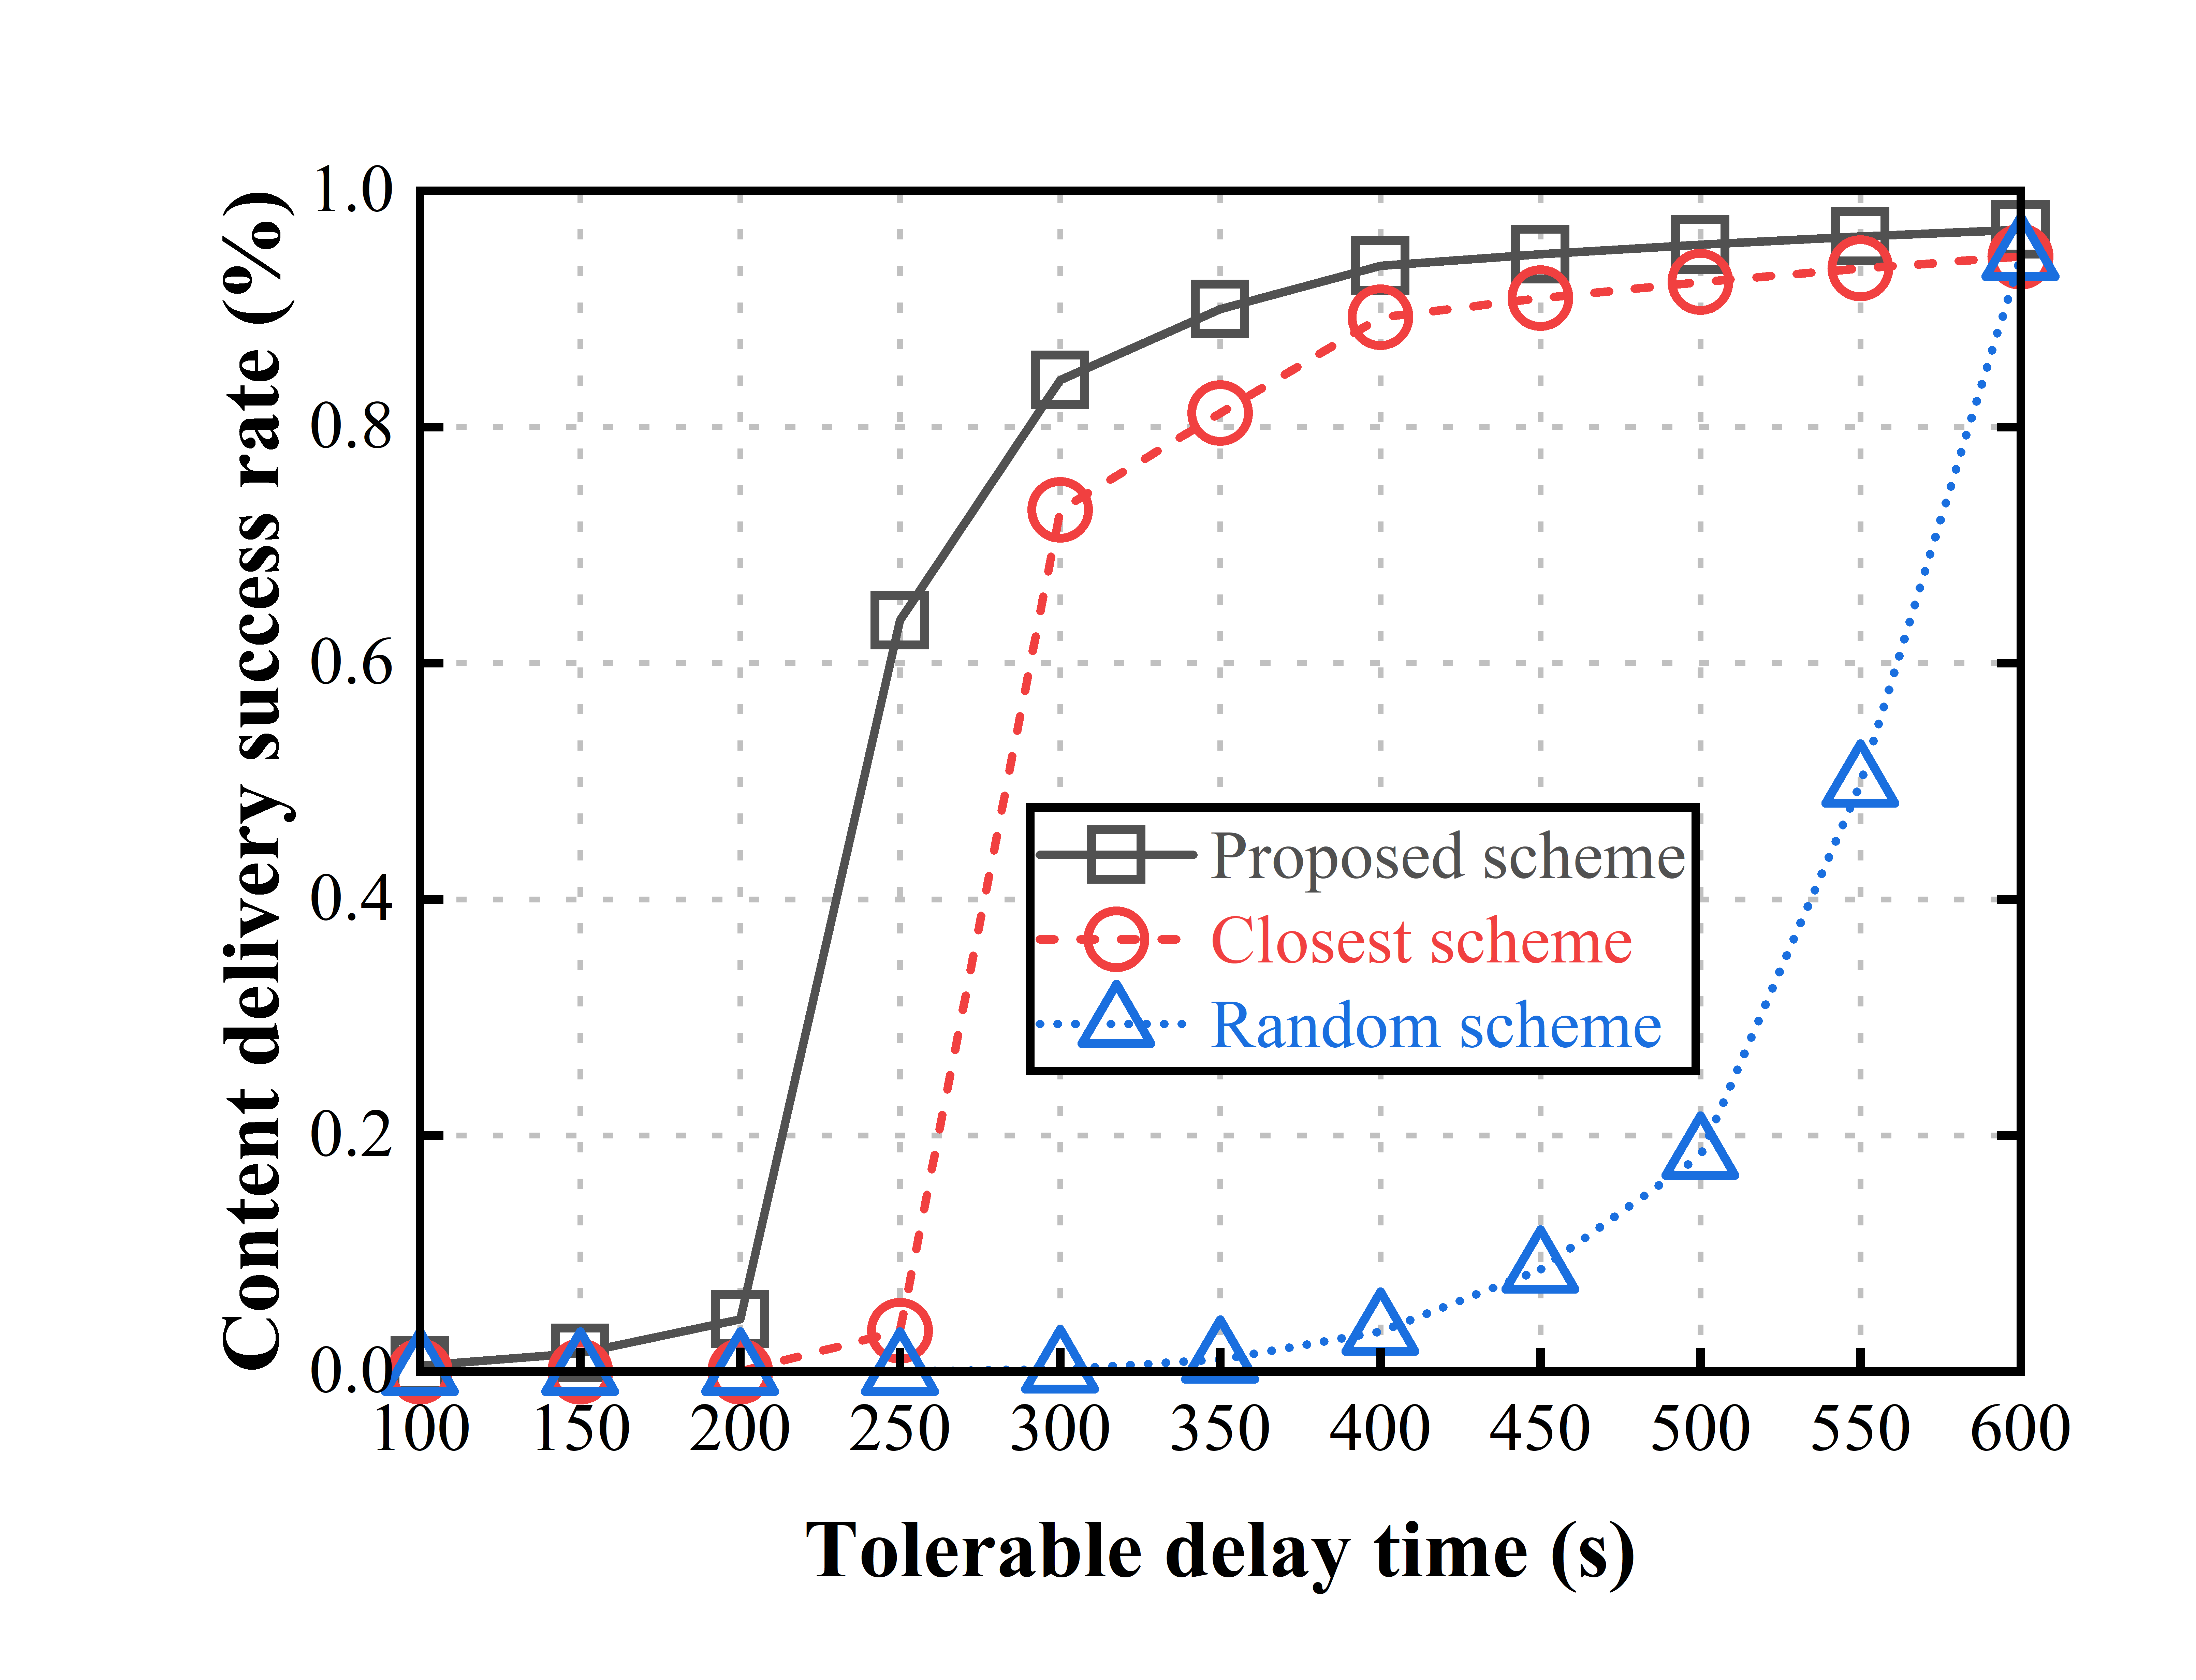
\includegraphics[width=0.48\textwidth]{./graph/Graph8.png}}
    \caption{According to the tolerable delay time: (a) the average burden; (b) the content delivery success rate.}
    \label{fig:g4}
\end{figure}

Figure \ref{fig:g4} demonstrates the performance for tolerable delay time to reflect various content.
The tolerable delay time affects the number of $PAR^{i,c}{k}$ that can be used as precaching RSUs.
Figure \ref{fig:g4}(a) shows the average burden according to the tolerable delay time.
When the tolerable delay time is very short, the average burden is high in all schemes because the number of $PAR^{i,c}_{k}$ is too small and the provision of $C_{c}$ has to be completed in the first RSU.
As the tolerable delay time increases, the number of $PAR^{i,c}_{k}$ increases.
The two comparison schemes do not consider tolerable delay time, so there is no performance impact.
As the number of $PAR^{i,c}_{k}$ increases in the proposed scheme, the number of RSUs to be selected as $OPR^{i,c}_{k}$ increases, leading to a significant performance improvement.

Figure \ref{fig:g4}(b) shows the content delivery success rate for tolerable delay time.
In the random scheme, the success rate increases as the tolerable delay time increases, due to a higher probability of randomly selected RSUs belonging to $PAR^{i,c}{k}$.
In the closest scheme, if there are too few $PAR^{i,c}_{k}$, the success rate is lower than the proposed scheme due to prediction error.
The success rate in the closest scheme improves as the number of $PAR^{i,c}{k}$ increases, reducing the impact of prediction error
In all schemes, the content is delivered with a high success rate when the number of $PAR^{i,c}_{k}$ is sufficiently high due to the very large tolerable delay time.
The proposed scheme increases the success rate by selecting better $ACR^{i,c}_{k}$ as $OPR^{i,c}_{k}$ when enough $PAR^{i,c}_{k}$ are available.

\section{Conclusion and Future Work} \label{sec.c}
The increased demand for contents due to the development of smart vehicles leads to significant mobile data traffics in content-centric vehicular networks (CCVNs).
Since a single RSU can't complete the provision of larger-sized content within its communication coverage, precaching content has been focused on as a solution.
Previous precaching schemes cost a lot of traffics to reduce delays by recklessly precaching contents in the next continuous RSUs on vehicles' trajectory with considering only delay-sensitive content.
By considering the already stored content on RSUs and the tolerable delay time that is decided by the content's characteristics, the traffic for precaching can be reduced.
Therefore, we propose a Traffic Optimized Content Precaching (TOCP) scheme in CCVN, which minimizes traffic consumption for delay-tolerant contents and decreases delay for delay-sensitive contents.
First, we denote a numerical model to decide to precache the requested content by the content provision calculation.
Then, we design packets for reducing the movements of large-size packets and updating the needed information, and also a Delay-tolerant content Management Model (DMM) for managing the updated information and conducting complex calculations.
Based on the updated information, we select optimal precaching RSUs by solving our optimization problem by using ILP.
Last, we provide a process for participating only selected OPRs in the content provision.
Simulation results demonstrate the scheme achieves minimizing caching and traffic burdens with a high content delivery success rate.
Taking into account the concept of DTC, this paper provides a promising foundation for developing an optimized precaching approach for both DSC and DTC in CCVN.

In our future work, we can consider other objective models or multi-objective models.
Firstly, more sophisticated algorithms can be developed to efficiently predict the tolerable delay time of various types of content based on their characteristics and user preferences.
Secondly, the proposed scheme can be extended to consider the context of vehicles such as their current location, destination, and speed, to improve the accuracy of the precaching decision.
Third, a versatile architecture can be designed by incorporating other schemes or precaching schemes for better delay-sensitive content.
Lastly, we can consider priori methods, posteriori methods, etc. to solve multi-objective models because there are many critical issues that have to be solved such as delays and reliability.

\begin{thebibliography}{00}
% Introduction
\bibitem{Zhe2020} Z. Zhang, C. -H. Lung, M. St-Hilaire and I. Lambadaris,  ``Smart Proactive Caching: Empower the Video Delivery for Autonomous Vehicles in ICN-Based Networks,'' \emph{IEEE Transactions on Vehicular Technology}, vol. 69, no. 7, pp. 7955--7965, Jul. 2020.
\bibitem{yuan2018} Q. Yuan, H. Zhou, J. Li, Z. Liu, F. Yang and X. S. Shen,  ``Toward Efficient Content Delivery for Automated Driving Services: An Edge Computing Solution,'' \emph{IEEE Network}, vol. 32, no. 1, pp. 80--86, Jan.-Feb. 2018.
\bibitem{Kumer2013} V. Kumar, S. Mishra and N. Chand,  ``Applications of VANETs: Present \& Future,'' \emph{Communications and Network}, vol. 5, no. 1B, pp. 12--15, Feb. 2013.
\bibitem{Pranav2019} P.K. Singh, S.K. Nandi and S. Nandi,  ``A tutorial survey on vehicular communication state of the art, and future research directions,'' \emph{Veh. Commun.}, vol. 18, pp. 100164, Aug. 2019.
\bibitem{Reichardt2002} D. Reichardt, M. Miglietta, L. Moretti, P. Morsink and W. Schulz,  ``CarTALK 2000: safe and comfortable driving based upon inter-vehicle-communication,'' \emph{Intelligent Vehicle Symposium, 2002. IEEE}, vol. 2, pp. 545--550, Jun. 2002.
\bibitem{Yen2020} Y. -T. Yen, J. -J. Chou, C. -S. Shih, C. -W. Chen and P. -K. Tsung,  ``Proactive Car-Following Using Deep-Reinforcement Learning,'' presented at the \emph{23\textsuperscript{rd} Int. Conf. Intelligent Transportation Systems}, Rhodes, Greece, Sep. 20--23, 2020.

% Traffic growth
\bibitem{Ericsson}
Ericsson Mobility Report. [Online]. Available: \underline{https://www.ericsson.com/en/reports--and--papers/mobility--report/}\\ \underline{dataforecasts/mobile--traffic--forecast}, Accessed on: Apr. 03, 2023.

\bibitem{Park2019} S. Park, S. Oh, Y. Nam, J. Bang and E. Lee,  ``Mobility-aware Distributed Proactive Caching in Content-Centric Vehicular Networks,'' presented at the \emph{12\textsuperscript{th} IFIP Wireless and Mobile Networking Conf.,} Paris, France, Sep. 11--13, 2019.

% precaching opt
\bibitem{Ahani2018} G. Ahani and D. Yuan, ``On Optimal Proactive and Retention-Aware Caching with User Mobility,'' presented at the \emph{88\textsuperscript{th} Vehicular Technology Conference (VTC-Fall)}, Chicago, IL, USA, 2018, pp. 1--5.
\bibitem{AlNagar2019} Y. AlNagar, S. Hosny and A. A. El-Sherif, ``Towards Mobility-Aware Proactive Caching for Vehicular Ad hoc Networks,'' \emph{2019 IEEE Wireless Communications and Networking Conference Workshop (WCNCW)}, Marrakech, Morocco, 2019, pp. 1--6.
\bibitem{Liang2018} C. Liang, F. R. Yu, N. Dao, G. Senarath and H. Farmanbar, ``Enabling Adaptive Data Prefetching in 5G Mobile Networks with Edge Caching,'' \emph{2018 IEEE Global Communications Conference (GLOBECOM)}, Abu Dhabi, United Arab Emirates, 2018, pp. 1--6.

% precaching learning
\bibitem{Hou2019} L. Hou, L. Lei, K. Zheng and X. Wang, ``A  $Q$ -Learning-Based Proactive Caching Strategy for Non-Safety Related Services in Vehicular Networks,'' \emph{IEEE Internet of Things Journal}, vol. 6, no. 3, pp. 4512--4520, June 2019.

% CCN
\bibitem{Jacobson2009} V. Jacobson, D.K. Smetters, J.D. Thornton, M.F. Plass, N.H. Briggs and R.L. Braynard,  ``Networking Named Content,'' presented at the \emph{5\textsuperscript{th} Int. Conf. Emerging networking experiments and technologies,} Rome, Italy, Dec. 1--4, 2009.
\bibitem{zhang2014} L. Zhang, A. Afanasyev, J. Burke, V. Jacobson, K. Claffy, P. Crowley, C. Papadopoulos, L. Wang and B. Zhang, ``Named data networking,'' \emph{ACM SIGCOMM Computer Communication Review}, vol. 44, no. 3, pp. 66-–73, Jul. 2014.


\bibitem{Khelifi2018} H. Khelifi, S. Luo, B. Nour, A. Sellami, H. Moungla and F. Naït-Abdesselam, ``An Optimized Proactive Caching Scheme Based on Mobility Prediction for Vehicular Networks,'' \emph{2018 IEEE Global Communications Conference}, Abu Dhabi, United Arab Emirates, Dec. 2018, pp. 1--6.

\bibitem{Zhu2019} Z. Zhu, Z. Zhang, W. Yan, Y. Huang and L. Yang, ``Proactive Caching in Auto Driving Scene via Deep Reinforcement Learning,'' presented at the \emph{11\textsuperscript{th} International Conference on Wireless Communications and Signal Processing}, Xi'an, China, 2019, pp. 1--6.

% ********** Related Work **********
% Precaching (Pop)
\bibitem{Ostrovskaya2018} S. Ostrovskaya et al.,  ``Towards Multi-metric Cache Replacement Policies in Vehicular Named Data Networks,'' presented at the \emph{29\textsuperscript{th} Annual Int. Symposium on Personal, Indoor and Mobile Radio Communications,} Bologna, Italy, Sep. 09--12, 2018.
\bibitem{Marica2021} M. Amadeo, G. Ruggeri, C. Campolo and A. Molinaro,  ``Diversity-improved caching of popular transient contents in Vehicular Named Data Networking,'' \emph{Comput. Netw}, vol. 184, pp. 107625, Jan. 2021.
\bibitem{Amit2019} A. Dua, M. Shishodia, N. Kumar, G. S. Aujla and N. Kumar,  ``Bloom Filter Based Efficient Caching Scheme for Content Distribution in Vehicular Networks,'' presented at the \emph{11\textsuperscript{th} Int. Conf. Communications Workshops,} Shanghai, China, May 20--24, 2019.

% DTC examples
\bibitem{Lee2014} E. Lee, E. Lee, M. Gerla and S. Y. Oh,  ``Vehicular cloud networking: architecture and design principles,'' \emph{IEEE Communications Magazine}, vol. 52, no. 2, pp. 148--155, Feb. 2014.
\bibitem{Chen2009} B. B. Chen and M. C. Chan,  ``MobTorrent: A Framework for Mobile Internet Access from Vehicles,'' \emph{IEEE INFOCOM}, Rio de Janeiro, Brazil, Apr. 2009, pp. 1404--1412.

% DTN
\bibitem{Qi2017} W. Qi, Q. Song, X. Wang and L. Guo ``Trajectory Data Mining-Based Routing in DTN-Enabled Vehicular Ad Hoc Networks,'' \emph{IEEE Access}, vol. 5, pp. 24128--24138, Oct. 2017.
\bibitem{Vigneri2019} L. Vigneri, T. Spyropoulos and C. Barakat ``Low Cost Video Streaming through Mobile Edge Caching: Modelling and Optimization,'' \emph{IEEE Transactions on Mobile Computing}, vol. 18, no. 6, pp. 1302--1315, Jun. 2019.
\bibitem{Xia2020} B. Xia, F. Kong, J. Zhou, X. Tang and H. Gong ``A Delay-Tolerant Data Transmission Scheme for Internet of Vehicles Based on Software Defined Cloud-Fog Networks,'' \emph{IEEE Access}, vol. 8, pp. 65911--65922, Mar. 2020.

\bibitem{Prates2019} A. A. Prates, I. V. Bastos and I. M. Moraes, ``GeoZone: An interest-packet forwarding mechanism based on dissemination zone for content-centric vehicular networks,'' \emph{Computers \& Electrical Engineering}, vol. 73, pp. 155--166, Jan. 2019.
\bibitem{Aung2023} N. Aung \emph{et al., ``}VeSoNet: Traffic-Aware Content Caching for Vehicular Social Networks Using Deep Reinforcement Learning,'' \emph{IEEE Transactions on Intelligent Transportation Systems}, to be published.


\bibitem{Amadeo2012} M. Amadeo, C. Campolo and A. Molinaro, ``Content-centric vehicular networking: An evaluation study,'' presented at the \emph{3\textsuperscript{rd} Int. Conf. the Network of the Future,} Tunis, Tunisia, Nov. 21--23, 2012.
\bibitem{Su2017} Z. Su, Y. Hui and Q. Yang,  ``The Next Generation Vehicular Networks: A Content-Centric Framework,'' \emph{IEEE Wireless Communications}, vol. 24, no. 1, pp. 60--66, Feb. 2017.
\bibitem{Wang2019} X. Wang and X. Wang, ``Vehicular Content-Centric Networking Framework,'' \emph{IEEE Systems Journal}, vol. 13, no. 1, pp. 519--529, Mar. 2019.
% \bibitem{Amadeo2012Crown} M. Amadeo, C. Campolo and A. Molinaro, ``CRoWN: Content-Centric Networking in Vehicular Ad Hoc Networks,'' \emph{IEEE Communications Lett.}, vol. 16, no. 9, pp. 1380--1383, Sep. 2012.
% \bibitem{Bouk2015} S. H. Bouk, S. H. Ahmed and D. Kim,  ``Vehicular content centric network (VCCN): a survey and research challenges,'' \emph{SAC '15: Proceedings of the 30th Annual ACM Symposium on Applied Computing}, Salamanca, Spain, Apr. 2015, pp. 695--700.
% \bibitem{Wang2017} M. Wang, C. Xu, S. Jia, J. Guan and L. A. Grieco ``Preference-aware Fast Interest Forwarding for video streaming in information-centric VANETs,'' presented at the \emph{2017 IEEE Int. Conf. Communications}, Paris, France, May 21--25, 2017.
% \bibitem{Rahman2018} F. H. Rahman, A. T. Wan, S. H. S. Newaz and W. S. Suhaili,  ``Vehicular Clustering: Fog Paradigm and Recent Advances,'' presented at the \emph{18\textsuperscript{th} Int. Conf. Communication Technology}, Chongqing, China, Oct. 08--11, 2018, pp. 468-472.

% Precaching
% \bibitem{Luo2020} Q. Luo, C. Li, T. H. Luan and W. Shi,  ``EdgeVCD: Intelligent Algorithm-Inspired Content Distribution in Vehicular Edge Computing Network,'' \emph{IEEE Internet of Things Journal}, vol. 7, no. 6, pp. 5562--5579, Jun. 2020.
% \bibitem{Lin2021} L. Yao, Y. Wang, X. Wang and G. WU,  ``Cooperative Caching in Vehicular Content Centric Network Based on Social Attributes and Mobility,'' \emph{IEEE Transactions on Mobile Computing},  vol. 20, no. 2, pp. 391--402, Feb. 2021.
% \bibitem{Kanai2016} K. Kanai et al.,  ``Proactive Content Caching for Mobile Video Utilizing Transportation Systems and Evaluation Through Field Experiments,'' \emph{IEEE Journal on Selected Areas in Communications}, vol. 34, no. 8, pp. 2102--2114, Aug. 2016.
% \bibitem{Yao2018} L. Yao, A. Chen, J. Deng, J. Wang and G. Wu,  ``A Cooperative Caching Scheme Based on Mobility Prediction in Vehicular Content Centric Networks,'' \emph{IEEE Transactions on Vehicular Technology}, vol. 67, no. 6, pp. 5435--5444, Jun. 2018.
% \bibitem{Zhou2019} H. Zhou, N. Cheng, J. Wang, J. Chen, Q. Yu and X. Shen,  ``Toward Dynamic Link Utilization for Efficient Vehicular Edge Content Distribution,'' \emph{IEEE Transactions on Vehicular Technology}, vol. 68, no. 9, pp. 8301--8313, Sep. 2019.
% \bibitem{Hui2020} H. Guo, L. Rui and Z. Gao,  ``A zone-based content pre-caching strategy in vehicular edge networks,'' \emph{Future Generation Computer Systems}, vol. 106, issue C, pp. 22--33, May 2020.
% \bibitem{Ahmed2021} A. Al-Hilo, D. Ebrahimi, S. Sharafeddine and C. Assi,  ``Vehicle-Assisted RSU Caching Using Deep Reinforcement Learning,'' \emph{IEEE Transactions on Emerging Topics in Computing (Early Access)}.
% \bibitem{Wang2021} R. Wang, Z. Kan, Y. Cui, D. Wu and Y. Zhen,  ``Cooperative Caching Strategy With Content Request Prediction in Internet of Vehicles,'' \emph{IEEE Internet of Things Journal}, vol. 8, no. 11, pp. 8964--8975, Jun. 2021.

% ********** Simulation **********
\bibitem{WAVE} % conference format in IEEE ACCESS
A. Paier \emph{et al., ``}Average Downstream Performance of Measured IEEE 802.11p Infrastructure-to-Vehicle Links,'' presented at the \emph{Int. Conf. Communications Workshops,} Cape Town, South Africa, May 23--27, 2010.

\bibitem{Zipf}
L. Breslau, Pei Cao, Li Fan, G. Phillips and S. Shenker, ``Web caching and Zipf-like distributions: evidence and implications,'' presented at the \emph{IEEE INFOCOM '99. Conference on Computer Communications. Proceedings. Eighteenth Annual Joint Conference of the IEEE Computer and Communications Societies. The Future is Now (Cat. No.99CH36320),} New York, NY, USA, Mar. 21--25, 1999, pp. 126-134, vol. 1.

\bibitem{NS3}
Network Simulator 3 (NS3). [Online]. Available: \underline{https://www.nsnam.org/}, Accessed on: Mar. 21, 2023.

\bibitem{Mangharam2006}
R. Mangharam, D. Weller, R. Rajkumar, P. Mudalige and F. Bai, ``GrooveNet: A Hybrid Simulator for Vehicle-to-Vehicle Networks,'' presented at the \emph{3\textsuperscript{rd} Annual Int. Conf. Mobile and Ubiquitous Systems: Networking \& Services}, San Jose, CA, USA, Jul. 17--21, 2006.

\bibitem{Sanguesa2013}
J. A. Sanguesa, M. Fogue, P. Garrido, F. J. Martinez, J.-C. Cano, C. T. Calafate and P. Manzoni. ``An Infrastructureless Approach to Estimate Vehicular Density in Urban Environments,'' \emph{Sensors}, vol. 13, no. 2, pp. 2399--2418, Feb. 2013.

\bibitem{Manhattan}
A. Hanggoro and R. F. Sari, ``Performance evaluation of the manhattan mobility model in vehicular ad-hoc networks for high mobility vehicle,'' presented at the \emph{2\textsuperscript{nd} Int. Conf. Communication, Networks and Satellite,} Yogyakarta, Indonesia, Dec. 03--04, 2013.

\bibitem{Nam2022} 
Y. Nam, J. Bang, J. Choi, Y. Shin and E. Lee, ``Cooperative Content Precaching Scheme Based on the Mobility Information of Vehicles in Intermittently Connected Vehicular Networks,'' \emph{Electronics}, vol. 11, no. 22, pp. 3663, Nov. 2022.

\bibitem{Wang2017} Y. Wang, Y. Liu, J. Zhang, H. Ye and Z. Tan, ``Cooperative Store–Carry–Forward Scheme for Intermittently Connected Vehicular Networks,'' \emph{IEEE Trans. Veh. Technol}, vol. 66, no. 1, pp. 777--784, Feb. 2016.

\end{thebibliography}

\begin{IEEEbiography}[{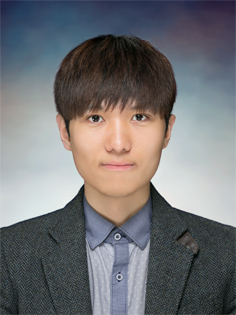
\includegraphics[width=1in,height=1.25in,clip,keepaspectratio]{./photo/YoungjuNam.jpg}}]
{Youngju Nam} received the B.S., M.S., and Ph.D. degrees from the School of Information and Communication Engineering, Chungbuk National University, Cheongju, South Korea, in 2017, 2019, and 2023, respectively. He is currently researching with the Research Institute for Computer and Information Communication, Chungbuk National University. His research interests include computer communication and networking, wireless sensor networks, content-centric vehicular networks, content precaching, optimization, and social networks.
\end{IEEEbiography}

\begin{IEEEbiography}[{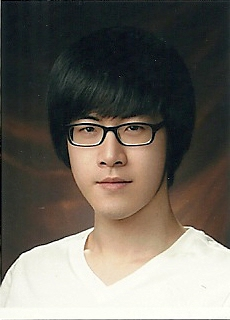
\includegraphics[width=1in,height=1.25in,clip,keepaspectratio]{./photo/HyunseokChoi.jpg}}]
{Hyunseok Choi} received the B.S. and Ph.D. degrees from the School of Information and Communication Engineering, Chungbuk National University, Cheongju, South Korea, in 2017 and 2023. He is currently researching with the Research Institute for Computer and Information Communication, Chungbuk National University. His research interests include computer communication and networking, wireless sensor networks, vehicular ad-hoc networks, vehicular clustering, and cloud computing.
\end{IEEEbiography}

\begin{IEEEbiography}[{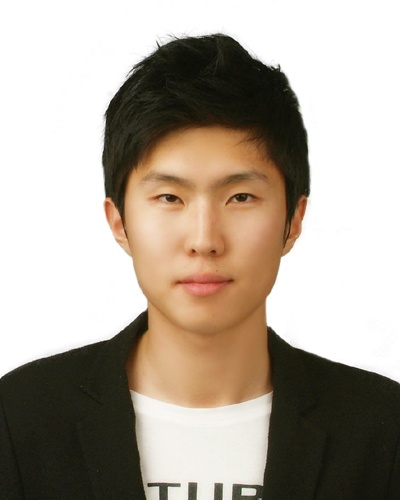
\includegraphics[width=1in,height=1.25in,clip,keepaspectratio]{./photo/YongjeShin.jpg}}]
{Yongje Shin} received the B.S., M.S., and Ph.D. degrees from the School of Information and Communication Engineering, Chungbuk National University,  Cheongju, South Korea, in 2016, 2018, and 2022, respectively. He is currently researching with the Research Institute for Computer and Information Communication, Chungbuk National University. His research interests include computer communication and networking, wireless sensor networks, vehicular ad-hoc networks, mobility management, and social intelligence networks.
\end{IEEEbiography}

\begin{IEEEbiography}[{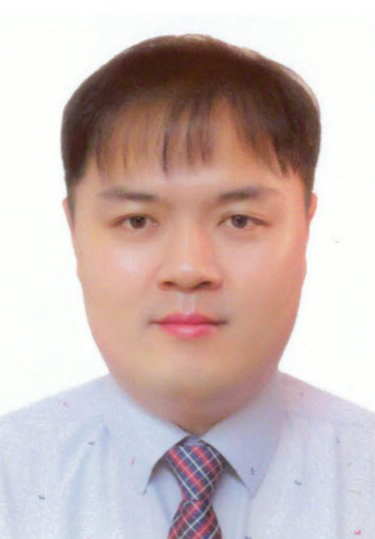
\includegraphics[width=1in,height=1.25in,clip,keepaspectratio]{./photo/SeungminOh.png}}]
{Seungmin Oh} (Member, IEEE) was born in Cheongju, Republic of Korea, in 1983. He received the B.S. and Ph.D. degrees in computer engineering from Chungnam National University, Republic of Korea, in 2009 and 2015, respectively. From 2016 to 2019, he was a Postdoctoral Researcher with the Network Research Laboratory, University of California at Los Angeles, Los Angeles. Since 2019, he has been an Assistant Professor with the Department of Computer Science and Engineering, Kongju National University. His research interests include routing protocols and applications for sensor networks, the Internet of Things (IoT), and internet of vehicles (IoV).
\end{IEEEbiography}


\begin{IEEEbiography}[{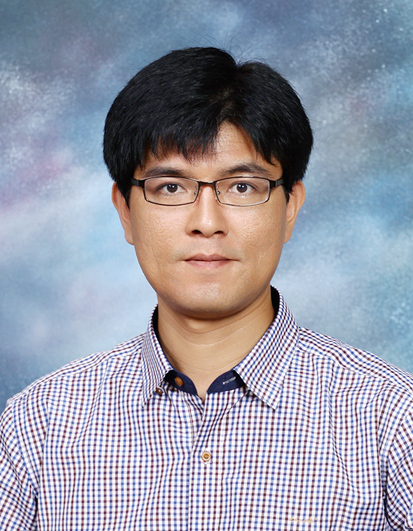
\includegraphics[width=1in,height=1.25in,clip,keepaspectratio]{./photo/EuisinLee.jpg}}]
{Euisin Lee} received the B.S., M.S., and Ph.D. degrees in computer engineering from Chungnam National University, Daejeon, South Korea, in 2005, 2007, and 2012, respectively. He studied as a Postdoctoral Researcher with the Department of Computer Science, University of California at Los Angeles, from 2012 to 2014. He joined the School of Information and Communication Engineering, Chungbuk National University, in 2014, where he is currently working as an Associate Professor. His research interests include computer communication and networking, routing, multicasting, mobility management, location service, QoS (real-time and reliability) in mobile ad hoc networks (MANETs), wireless sensor networks (WSNs), vehicular ad hoc networks (VANETs), and smart grid. 
\end{IEEEbiography}

\EOD
\end{document}
